% Cours et préparation aux entretiens du projet PPA Pricer.
% Compilation : cd docs/cours && tectonic cours_ppa.tex
% (ou xelatex / pdflatex, deux passes pour la table des matières)
\documentclass[11pt,a4paper]{article}

\usepackage{iftex}
\ifPDFTeX
  \usepackage[T1]{fontenc}
  \usepackage{lmodern}
\else
  \usepackage{fontspec}
\fi
\usepackage[french]{babel}
\usepackage{microtype}
\usepackage[margin=2.4cm]{geometry}
\usepackage{amsmath,amssymb}
\usepackage{booktabs,tabularx,array}
\usepackage{graphicx}
\usepackage{float}
\usepackage[titles]{tocloft}
\setlength{\cftbeforesecskip}{4pt}
\usepackage{xcolor}
\usepackage[most]{tcolorbox}
\usepackage{listings}
\usepackage{enumitem}
\usepackage{tikz}
\usetikzlibrary{arrows.meta,positioning,babel}
\usepackage[hidelinks]{hyperref}

\graphicspath{{../../reports/analyse/}}
\setlist{itemsep=2pt,topsep=4pt}
\setlength{\parskip}{4pt}
\setlength{\parindent}{0pt}
\newcolumntype{Y}{>{\raggedright\arraybackslash}X}
\renewcommand{\arraystretch}{1.15}

\definecolor{bleu}{HTML}{2A78D6}
\definecolor{orange}{HTML}{EB6834}
\definecolor{vert}{HTML}{1BAF7A}
\definecolor{gris}{HTML}{6B7280}

\tcbset{commun/.style={breakable,enhanced,boxrule=0.4pt,arc=2pt,left=7pt,right=7pt,top=4pt,bottom=4pt,
  fonttitle=\bfseries\small,before skip=8pt,after skip=8pt}}
\newtcolorbox{aretenir}{commun,colback=bleu!5,colframe=bleu!80!black,title={À retenir}}
\newtcolorbox{attention}{commun,colback=orange!6,colframe=orange!85!black,title={Attention}}
\newtcolorbox{entretien}{commun,colback=vert!6,colframe=vert!70!black,title={À dire en entretien}}
\newtcolorbox{pascode}{commun,colback=gris!8,colframe=gris,title={Pas encore codé}}
\newtcolorbox{definition}[1]{commun,colback=white,colframe=gris!70,title={#1}}

\newcommand{\code}[1]{\texttt{\small #1}}
\newcommand{\TC}{\mathrm{TC}}
\newcommand{\Cov}{\mathrm{Cov}}
\newcommand{\MAE}{\mathrm{MAE}}
\newcounter{qr}
\newcommand{\qr}[2]{\stepcounter{qr}\par\medskip\noindent\textbf{Q\theqr.\ #1}\par\nopagebreak\noindent #2\par}
\newcounter{exo}
% L'énoncé s'affiche sur place ; le corrigé est mis de côté et imprimé par \corriges, dans la section Corrigés.
\newcommand{\lescorriges}{}
\newcommand{\corrigeexo}[2]{\par\medskip\noindent\textbf{Exercice #1.} #2\par}
\newcommand{\exo}[2]{\stepcounter{exo}\par\medskip\noindent\textbf{Exercice \theexo.} #1\par
  \xdef\lescorriges{\unexpanded\expandafter{\lescorriges}\noexpand\corrigeexo{\theexo}{\unexpanded{#2}}}}
\newcommand{\corriges}{\lescorriges}
\newtcolorbox{demo}[1]{commun,colback=white,colframe=bleu!45,title={Démonstration : #1}}

\lstset{language=Python,basicstyle=\ttfamily\footnotesize,keywordstyle=\color{bleu!80!black}\bfseries,
  commentstyle=\color{gris}\itshape,stringstyle=\color{orange!85!black},showstringspaces=false,
  breaklines=true,frame=single,framerule=0.3pt,rulecolor=\color{gris!50},xleftmargin=4pt,xrightmargin=4pt,
  columns=fullflexible,keepspaces=true,
  literate={é}{{\'e}}1 {è}{{\`e}}1 {ê}{{\^e}}1 {à}{{\`a}}1 {ç}{{\c{c}}}1 {ù}{{\`u}}1 {î}{{\^i}}1 {ô}{{\^o}}1}
% Un extrait de code reste entier sur une page.
\lstnewenvironment{codepy}{\endgraf\noindent\minipage{\linewidth}}{\endminipage\endgraf}

\title{\textbf{PPA solaires en France}\\[4pt]\large Cours technique et préparation aux entretiens}
\author{Projet PPA Pricer --- Jean-Baptiste Bourrée}
\date{Version du 30 octobre 2026}

\begin{document}
\maketitle

\begin{abstract}
\noindent Ce document explique de bout en bout le projet : le marché, les PPA, les données, le modèle, le
backtest et ce qu'il reste à faire. Les encadrés verts donnent ce qu'il faut savoir dire à l'oral, et une section regroupe 41 questions probables.
Les chiffres viennent des rapports du projet (\code{reports/}, générés les 29 et 30/10/2026). Les
parties sur le fonctionnement du marché relèvent de connaissances générales et n'ont pas été
vérifiées avec les données du projet : à recouper avant de les citer avec précision.
\end{abstract}

\setcounter{tocdepth}{1}
\tableofcontents
\newpage

% ====================================================================
\section{L'essentiel, à relire la veille}

\subsection{Le pitch}

\begin{entretien}
\textbf{En 30 secondes.} J'ai construit en Python un outil qui prévoit le taux de capture solaire
mensuel en France, c'est-à-dire le prix réellement obtenu par le solaire rapporté au prix moyen du
marché. C'est le paramètre clé du prix d'un PPA pay-as-produced. J'ai figé le protocole avant de voir
les résultats, puis testé le modèle sur 8 ans hors échantillon contre deux références naïves. Il les
bat, mais son avantage sur la plus forte n'est pas significatif, et il surestime nettement le taux de
capture depuis 2024. Les versions suivantes réduisent cette erreur sans la faire disparaître.

\medskip
\textbf{Si on me demande plus.} Le taux de capture est passé de 102\,\% en 2018 à 59\,\% en 2025 : le
solaire fait baisser le prix aux heures où il produit. Mon modèle est une régression du taux de
capture sur la part du solaire, avec un effet par mois. Pour chaque année de 2018 à 2025, il est
calibré uniquement sur le passé. En testant la plausibilité physique des données, j'ai aussi trouvé
un décalage d'environ une heure dans la production solaire publiée, invisible pour les contrôles
classiques. Il ne change pas le verdict. Pour une livraison 2027 à Montpellier, ancrée sur une cotation de 122,6~€/MWh, j'obtiens environ 71~€/MWh, dans une fourchette de 60 à 84, avant garanties d'origine, équilibrage, crédit et marge. Ce prix suit la cotation, et la moitié du revenu vient du premier trimestre.
\end{entretien}

\subsection{Les chiffres à connaître}

\begin{center}
\begin{tabularx}{\linewidth}{Yl}
\toprule
\textbf{Grandeur} & \textbf{Valeur} \\
\midrule
Taux de capture annuel, 2018 $\to$ 2025 & 102,1\,\% $\to$ 58,8\,\% \\
Part du solaire dans la consommation, 2018 $\to$ 2025 & 2,1\,\% $\to$ 6,9\,\% \\
Heures à prix négatif, 2018 $\to$ 2025 ; 2026 au 30/10 & 11 $\to$ 513 ; 565 \\
Solaire produit à prix négatif en 2025 & 15,7\,\% de l'énergie \\
MAE 2018--2025 : modèle / R1 / R2 (points de taux de capture) & 5,9 / 6,6 / 11,2 \\
Skill score du modèle contre R1 / contre R2 & $+0{,}10$ / $+0{,}47$ \\
p-value Diebold-Mariano contre R1 / contre R2 & 0,449 / 0,007 \\
Erreur sur le taux de capture annuel 2025 & $+13{,}3$ points \\
Prix rétrospectif 2025 : prévu / réalisé & 44,0 / 35,9 €/MWh \\
Pente $\hat\beta$ selon l'année de calibration & de $-2{,}86$ à $-6{,}22$ \\
Mois signalés par le contrôle de calage (sur 142) & 20 décalés, 13 avec solaire de nuit \\
Taux de capture 2025 : Energy-Charts / RTE & 58,81\,\% / 56,04\,\% \\
Valeur 2027, baseload de 61~€/MWh : V1 / persistance & 32,4 / 37,1 €/MWh \\
Valeur 2027, courbe à terme, 40~GW : V2 / persistance & 70,6 / 74,0 €/MWh \\
VaR à 95\,\% du spot, sur la courbe, pour 1~MWc & 44\,500~€, 50\,\% du revenu moyen \\
\bottomrule
\end{tabularx}
\end{center}

\subsection{Les cinq idées clés}

\begin{enumerate}
\item Un PPA pay-as-produced vaut environ \emph{baseload futur $\times$ taux de capture futur}.
\item Le taux de capture est bas quand production solaire et prix sont négativement corrélés. Le parc y contribue, mais il
n'explique pas tout : la chute de 2024 reste non établie dans mes tests.
\item Un backtest honnête se juge contre des références simples, sur des données absentes de l'estimation, avec un
protocole figé à l'avance.
\item Un skill score positif ne suffit pas : il faut aussi tester la significativité, et regarder où
les erreurs se concentrent.
\item Des contrôles de données « tous à zéro » ne garantissent pas que les données sont justes.
\end{enumerate}

\begin{attention}
Le pricing V1 (section~\ref{sec:pricing}) donne une \textbf{valeur de l'énergie au spot sur un an}, pas un prix de
contrat. Côté stochastique, M0, M1 et M2 sont codés, et aucun ne remplit le critère du protocole : M2 fait seulement jeu égal avec la V1. Le prix de référence pour 2027 vient de la V2, dont la forme reste à juger sur des mois nouveaux. Le Monte-Carlo, la VaR et les contrats baseload et avec plancher sont codés sur un an seulement, et la VaR est un ordre de grandeur. Une appli Streamlit privée reprend ces calculs (section~\ref{sec:formules}). Les contrats pluriannuels ne sont pas codés. Ne pas les présenter comme faits.
\end{attention}

% ====================================================================
\section{Le marché de l'électricité}

\subsection{Puissance et énergie}

La \textbf{puissance} (MW) est un débit ; l'\textbf{énergie} (MWh) est une quantité. Un parc de 1~MW qui
tourne à plein pendant 1~h produit 1~MWh. Un prix s'exprime en €/MWh. Ordres de grandeur du projet : le
solaire français a produit environ 30~TWh en 2025, soit 3,4~GW en moyenne sur l'année, avec des pointes
bien plus élevées à midi.

L'électricité se stocke mal à grande échelle : l'offre doit égaler la demande à chaque instant. D'où des
prix très variables d'une heure à l'autre, que l'on n'observe pas sur une action.

\subsection{Les marchés, du plus lointain au plus proche}

\begin{center}
\begin{tabularx}{\linewidth}{>{\raggedright\arraybackslash}p{3.6cm}YY}
\toprule
\textbf{Marché} & \textbf{Ce qu'on y échange} & \textbf{Dans le projet} \\
\midrule
À terme (EEX) & Livraison future : mois, trimestre, année, en baseload ou en pointe & Payant ; cotations relevées sur une source secondaire (H19) \\
Day-ahead (EPEX SPOT, Nord Pool) & Enchère la veille, pour chaque période du lendemain & Donnée centrale du projet \\
Infrajournalier & Ajustements en continu et par enchères jusque peu avant la livraison & Non utilisé \\
Équilibrage (RTE) & Le gestionnaire de réseau corrige les derniers écarts & Non utilisé en V1 \\
\bottomrule
\end{tabularx}
\end{center}

\textbf{Baseload} (ou ruban) : même puissance à toutes les heures. Le prix baseload d'une période est la
moyenne simple des prix. \textbf{Peakload} : même chose sur les heures de pointe, conventionnellement de
8~h à 20~h en semaine.

\subsection{L'enchère day-ahead}

Chaque jour vers 12~h, les acteurs déposent leurs offres pour le lendemain. Les marchés européens sont
couplés (\emph{Single Day-Ahead Coupling}) : l'algorithme calcule un prix par zone en tenant compte des
capacités d'échange entre pays. La France forme une seule zone de prix.

Le prix est \textbf{marginal et uniforme} (\emph{pay-as-clear}) : tous les producteurs retenus reçoivent le
prix de la dernière offre nécessaire pour couvrir la demande. Ce mécanisme s'appelle le \textbf{merit
order} : on empile les moyens de production du moins cher au plus cher, en coût marginal.

\begin{figure}[ht]
\centering
\begin{tikzpicture}[x=0.5cm,y=0.75cm,font=\footnotesize]
  \newcommand{\bloc}[5]{\fill[#5] (#1,0) rectangle (#2,#3); \draw[white,line width=0.8pt] (#1,0) rectangle (#2,#3); \node[align=center] at ({(#1+#2)/2},#3+0.25) {#4};}
  \begin{scope}
    \bloc{0}{1.2}{0.1}{Sol.}{vert}
    \bloc{1.2}{4.8}{0.5}{Nucléaire}{bleu!55}
    \bloc{4.8}{6.6}{1.0}{Hydro}{bleu!30}
    \bloc{6.6}{8.6}{2.2}{Gaz}{orange!70}
    \bloc{8.6}{10}{3.0}{Fioul}{orange!40}
    \draw[-{Latex}] (0,0) -- (10.8,0);
    \draw[-{Latex}] (0,0) -- (0,3.9) node[right] {coût marginal};
    \node[anchor=north] at (5.4,-0.05) {capacité cumulée};
    \draw[thick,dashed] (6.85,0) -- (6.85,3.5) node[above] {demande};
    \draw[thick,red!70!black] (0,2.2) -- (6.85,2.2);
    \node[red!70!black,anchor=south west] at (0.1,2.2) {prix élevé};
    \node at (5.4,-0.95) {\textbf{Peu de solaire} : le gaz fixe le prix};
  \end{scope}
  \begin{scope}[xshift=7.6cm]
    \bloc{0}{3.5}{0.1}{Solaire}{vert}
    \bloc{3.5}{7}{0.5}{Nucléaire}{bleu!55}
    \bloc{7}{8.8}{1.0}{Hydro}{bleu!30}
    \bloc{8.8}{10.8}{2.2}{Gaz}{orange!70}
    \draw[-{Latex}] (0,0) -- (11.6,0);
    \draw[-{Latex}] (0,0) -- (0,3.9) node[right] {coût marginal};
    \node[anchor=north] at (5.8,-0.05) {capacité cumulée};
    \draw[thick,dashed] (6.85,0) -- (6.85,3.5) node[above] {demande};
    \draw[thick,red!70!black] (0,0.5) -- (6.85,0.5);
    \node[red!70!black,anchor=south west] at (0.1,1.0) {prix bas};
    \node at (5.8,-0.95) {\textbf{Beaucoup de solaire} : l'empilement glisse};
  \end{scope}
\end{tikzpicture}
\caption{Schéma du merit order, sans données réelles. À midi, le solaire au coût marginal quasi nul
décale l'empilement vers la droite : à demande égale, le prix baisse.}
\end{figure}

Le pas de temps du day-ahead est passé à 15~minutes pour la livraison du 1\textsuperscript{er} octobre 2025
(constaté dans nos données, hypothèse H1).

\subsection{Pourquoi des prix négatifs}

Un prix négatif signifie qu'un producteur paie pour produire. Cela arrive quand l'offre rigide dépasse la
demande et les capacités d'export : un réacteur coûte cher à arrêter puis à relancer, et une partie du
renouvelable peut être soutenue sans lien direct avec le prix de marché, même si des contrats récents suspendent ce soutien aux prix négatifs. Ces producteurs préfèrent accepter un prix
négatif plutôt que de s'arrêter. Le plancher harmonisé de l'enchère européenne est de $-500$~€/MWh ; le prix
horaire le plus bas de nos données est de $-497$~€/MWh.

\begin{aretenir}
\begin{itemize}[leftmargin=*]
\item Le prix day-ahead est fixé par la dernière unité appelée, pas par le coût moyen.
\item Baseload = moyenne simple des prix. Un producteur solaire ne touche pas ce prix-là.
\item Prix négatif = offre rigide excédentaire, pas une erreur de données.
\end{itemize}
\end{aretenir}

% ====================================================================
\section{Les PPA}

\subsection{Définition}

Un \textbf{PPA} (\emph{Power Purchase Agreement}) est un contrat long terme, de quelques années à 20~ans, par lequel un
producteur vend l'électricité d'un parc à un acheteur (entreprise, fournisseur) à un prix convenu à l'avance.
Le producteur sécurise un revenu qui facilite le financement du parc ; l'acheteur fixe une partie de son
coût d'énergie et obtient souvent les \textbf{garanties d'origine} (certificats attestant l'origine renouvelable).

\begin{itemize}
\item \textbf{Physique} : l'électricité est livrée à l'acheteur via le réseau.
\item \textbf{Financier} (ou virtuel) : chacun reste sur le marché et l'on règle seulement la différence entre
le prix fixe et un prix de référence.
\end{itemize}

\subsection{Les structures, et qui porte quel risque}

Notons $K$ le prix fixe, $q_t$ la production et $p_t$ le prix spot.

\begin{center}
\begin{tabularx}{\linewidth}{lYY}
\toprule
\textbf{Structure} & \textbf{Fonctionnement} & \textbf{Qui porte quoi} \\
\midrule
Pay-as-produced & L'acheteur paie $K$ pour chaque MWh réellement produit & L'acheteur porte le profil et doit couvrir un volume variable ; le revenu du vendeur reste lié à sa production \\
Baseload & Le vendeur livre un ruban constant $V$ au prix $K$, et achète ou vend l'écart au spot & Le vendeur porte le volume et le profil \\
Avec plancher & Le vendeur touche au moins $K_f$ par MWh, avant la prime & Le coût du plancher est une option, à payer \\
\bottomrule
\end{tabularx}
\end{center}

Le résultat de l'acheteur d'un pay-as-produced, comparé à un achat au spot, est $\sum_t q_t\,(p_t - K)$.

\subsection{Les cinq risques}

\begin{itemize}
\item \textbf{Prix} : le niveau général du marché (le baseload) change.
\item \textbf{Profil} : le solaire capte moins que le baseload. C'est le taux de capture, cœur du projet.
\item \textbf{Volume} : l'ensoleillement ou la disponibilité du parc diffèrent de la prévision.
\item \textbf{Équilibrage} : l'écart entre production prévue et réalisée est facturé au prix des écarts.
\item \textbf{Contrepartie} : l'autre partie peut faire défaut sur un contrat de plusieurs années.
\end{itemize}

Les trois premiers s'écrivent comme une somme de logarithmes, mais leurs risques ne s'additionnent pas simplement, car ils sont corrélés. Pour un an de production $Q$ :
\[
\text{Revenu au spot} = Q \times B \times \TC
\qquad\text{donc}\qquad
\ln(\text{Revenu}) = \ln Q + \ln B + \ln \TC .
\]

\subsection{Le prix juste}

Un PPA pay-as-produced est au prix juste quand sa valeur espérée actualisée est nulle, avec $D_t$ le facteur d'actualisation :
\[
\mathbb{E}\Big[\sum_t D_t\, q_t\,(p_t - K)\Big] = 0
\quad\Longrightarrow\quad
K^\star = \frac{\mathbb{E}\big[\sum_t D_t\, q_t\, p_t\big]}{\mathbb{E}\big[\sum_t D_t\, q_t\big]} .
\]
C'est un prix capté espéré. Sur une période courte, en ignorant les primes et le lien entre baseload et taux de capture, $K^\star \approx B \times \TC$. Le vrai
prix d'un contrat ajoute les garanties d'origine, les coûts d'équilibrage, le risque de crédit et la marge.

\subsection{Un résultat utile : le baseload ne supprime pas la cannibalisation}

Un vendeur livre un ruban $V$ au prix $K$ et règle l'écart au spot. Son revenu est
$\sum_t [V K + (q_t - V)\,p_t]$. Avec $V = \bar q$ (même énergie totale) et $K = B$, les termes en $V$ s'annulent :
\[
\sum_t \big[\bar q\, B + (q_t - \bar q)\,p_t\big] = N\bar q B + \sum_t q_t p_t - \bar q\, N B = \sum_t q_t p_t .
\]
Si $K$ égale le baseload réalisé, il reçoit donc exactement le prix capté $C$ par MWh ; sinon, il reçoit $C + K - B$. La structure baseload ne fait pas disparaître le risque de
profil : elle le laisse au vendeur.

\begin{aretenir}
\begin{itemize}[leftmargin=*]
\item Pay-as-produced : le risque de profil passe à l'acheteur, qui doit aussi couvrir un volume variable ; le revenu du vendeur reste lié à sa production.
\item Baseload : il reste au vendeur.
\item Prix juste $\approx$ baseload $\times$ taux de capture, avant coûts et primes.
\end{itemize}
\end{aretenir}

% ====================================================================
\section{Le taux de capture et la cannibalisation}

\subsection{Définitions}

Pour une période (mois ou année), avec $p_h$ le prix et $q_h$ la production solaire nationale de l'heure $h$ :

\begin{definition}{Les quatre grandeurs du projet}
\[
B = \frac{1}{N}\sum_h p_h,
\qquad
C = \frac{\sum_h q_h\,p_h}{\sum_h q_h},
\qquad
\TC = \frac{C}{B},
\qquad
S = \frac{\sum_h q_h}{\sum_h \mathrm{conso}_h}.
\]
$B$ : baseload. $C$ : prix capté. $\TC$ : taux de capture. $S$ : part du solaire.
\end{definition}

\textbf{Exemple réel, le 15 juin 2025.} À minuit, le prix est de 51,4~€/MWh sans soleil ; à 13~h, il tombe à
$-5{,}6$~€/MWh avec 8\,323~MW de solaire. Sur la journée, $B = 17{,}44$, $C = 2{,}88$ et $\TC = 16{,}5\,\%$.

\textbf{Vérification sur juin 2025.} La fonction du projet et le calcul à la main donnent $B = 40{,}74$,
$C = 19{,}99$, $\TC = 49{,}07\,\%$ et $S = 12{,}03\,\%$.

\subsection{La cannibalisation est une covariance}

En développant $\frac1N\sum_h q_h p_h = \Cov(q,p) + \bar q\,\bar p$ et en divisant par $\bar q$ :
\[
C = B + \frac{\Cov(q,p)}{\bar q}
\qquad\Longrightarrow\qquad
\boxed{\ \TC = 1 + \frac{\Cov(q,p)}{\bar q\;\bar p}\ }
\]
Le taux de capture est inférieur à 100\,\% exactement quand production et prix sont négativement corrélés. Sur
2025, nos données donnent une corrélation de $-0{,}40$, et cette identité redonne bien 58,81\,\%.

Un taux au-dessus de 100\,\% peut avoir deux causes. \emph{Dans le mois} : de 2015 à 2019, la moyenne des taux mensuels pondérée par l'énergie dépasse 100\,\%, car la demande de journée rendait midi plus cher que la nuit. \emph{Entre les mois} : le 105,7\,\% de 2022 vient d'un été très cher, alors que cette moyenne mensuelle n'y vaut que 97,4\,\%. Le taux chute ensuite nettement en 2024, sans que mes tests en établissent toute la cause.

\subsection{Le taux annuel n'est pas la moyenne des mois}

Le prix capté annuel est pondéré par l'énergie. Avec $w_m = Q_m / \sum_k Q_k$ :
\[
\TC_{\text{an}} = \frac{\sum_m w_m\,\TC_m\,B_m}{B_{\text{an}}}
\qquad\text{où}\qquad
B_{\text{an}} = \frac{\sum_m B_m H_m}{\sum_m H_m}.
\]
Sur 2025 : la moyenne simple des 12 mois donne 65,6\,\% ; pondérer par l'énergie donne 58,0\,\% ; la formule
complète donne \textbf{58,8\,\%}. Les mois très solaires ont un taux faible et pèsent plus, comme dans le revenu réel d'un parc.

\begin{center}
\small
\begin{tabular}{lrrrrr}
\toprule
\textbf{2025} & $B$ (€/MWh) & $C$ (€/MWh) & $\TC$ (\%) & $S$ (\%) & Solaire (GWh) \\
\midrule
Janvier & 102,3 & 105,9 & 103,6 & 2,1 & 1\,047 \\
Février & 122,7 & 111,0 & 90,5 & 3,7 & 1\,545 \\
Mars & 76,9 & 49,9 & 64,9 & 6,5 & 2\,603 \\
Avril & 42,2 & 17,1 & 40,5 & 8,8 & 2\,837 \\
Mai & 19,4 & 4,0 & 20,9 & 10,9 & 3\,300 \\
Juin & 40,7 & 20,0 & 49,1 & 12,0 & 3\,748 \\
Juillet & 58,0 & 38,3 & 66,1 & 12,6 & 4\,063 \\
Août & 54,4 & 26,1 & 47,9 & 12,0 & 3\,629 \\
Septembre & 34,8 & 17,4 & 49,9 & 8,7 & 2\,675 \\
Octobre & 57,5 & 44,0 & 76,5 & 6,7 & 2\,291 \\
Novembre & 59,1 & 48,7 & 82,3 & 3,5 & 1\,370 \\
Décembre & 68,6 & 64,9 & 94,7 & 2,5 & 1\,093 \\
\bottomrule
\end{tabular}
\end{center}

\subsection{Les choix de calcul}

\begin{center}
\begin{tabularx}{\linewidth}{YYY}
\toprule
\textbf{Choix} & \textbf{Pourquoi} & \textbf{Sur nos données} \\
\midrule
Mois et années de Paris & Convention des contrats & Écart avec des mois UTC : 0,08 point en moyenne, 0,31 au plus \\
Mêmes heures pour tout & Une heure chère sans solaire connu gonflerait $B$ seul & Couvert par un test \\
Période invalide au-delà de 5\,\% d'heures manquantes & Pas de ratio sur une période trop incomplète & Janv. 2015 (12,9\,\%), oct. 2026 (7,8\,\%, mois en cours), année 2026 \\
Prix négatifs comptés (H3) & Le contrat paie la production même à prix négatif & 2025 : 58,8\,\%, contre 60,8\,\% avec un plancher à 0 \\
\bottomrule
\end{tabularx}
\end{center}

\begin{attention}
Le taux de capture est un ratio : il devient fragile quand $B$ est faible. En mai 2025, $B = 19{,}4$~€/MWh et
$\TC = 20{,}9\,\%$. Un écart de quelques €/MWh sur $C$ y pèse beaucoup en points. De plus, le plancher à 0 ci-dessus
est une simple sensibilité : un vrai arrêt de production changerait aussi les volumes.
\end{attention}

\subsection{Ce que montrent les données}

\begin{center}
\small
\begin{tabular}{lrrrrr}
\toprule
\textbf{Année} & $B$ (€/MWh) & $C$ (€/MWh) & $\TC$ (\%) & $S$ (\%) & Heures $p<0$ \\
\midrule
2015 & 38,5 & 39,3 & 102,1 & 1,5 & 0 \\
2016 & 36,7 & 34,8 & 94,6 & 1,7 & 2 \\
2017 & 45,0 & 41,4 & 92,1 & 1,9 & 4 \\
2018 & 50,2 & 51,3 & 102,1 & 2,1 & 11 \\
2019 & 39,4 & 37,7 & 95,7 & 2,4 & 27 \\
2020 & 32,2 & 29,9 & 92,7 & 2,8 & 102 \\
2021 & 109,2 & 94,2 & 86,3 & 2,9 & 64 \\
2022 & 275,8 & 291,5 & 105,7 & 4,0 & 4 \\
2023 & 96,9 & 83,6 & 86,3 & 5,1 & 147 \\
2024 & 58,0 & 39,2 & 67,6 & 5,4 & 352 \\
2025 & 61,1 & 35,9 & 58,8 & 6,9 & 513 \\
\bottomrule
\end{tabular}
\end{center}

\begin{enumerate}
\item \textbf{La cannibalisation est forte et récente} : de 86 à 106\,\% jusqu'en 2023, puis 68\,\% en 2024 et 59\,\% en 2025.
\item \textbf{La relation n'est pas linéaire et dépend de la saison} : au printemps, $\TC$ tombe à 10--30\,\% pour
$S$ de 10--13\,\% (avril--mai 2025--2026), alors qu'en été il reste autour de 50--65\,\% pour une part comparable.
\item \textbf{Le creux de midi se creuse brutalement en 2024} : au printemps, le prix de 14~h vaut 0,72 fois le prix moyen de l'année en 2023, 0,25 en 2024 et 0,11 en 2025, contre 0,7 à 0,9 avant 2019.
\item \textbf{Les prix négatifs explosent} : 11~heures en 2018, 513 en 2025, déjà 565 en 2026 au 30/10.
\end{enumerate}

\begin{figure}[!ht]
\centering
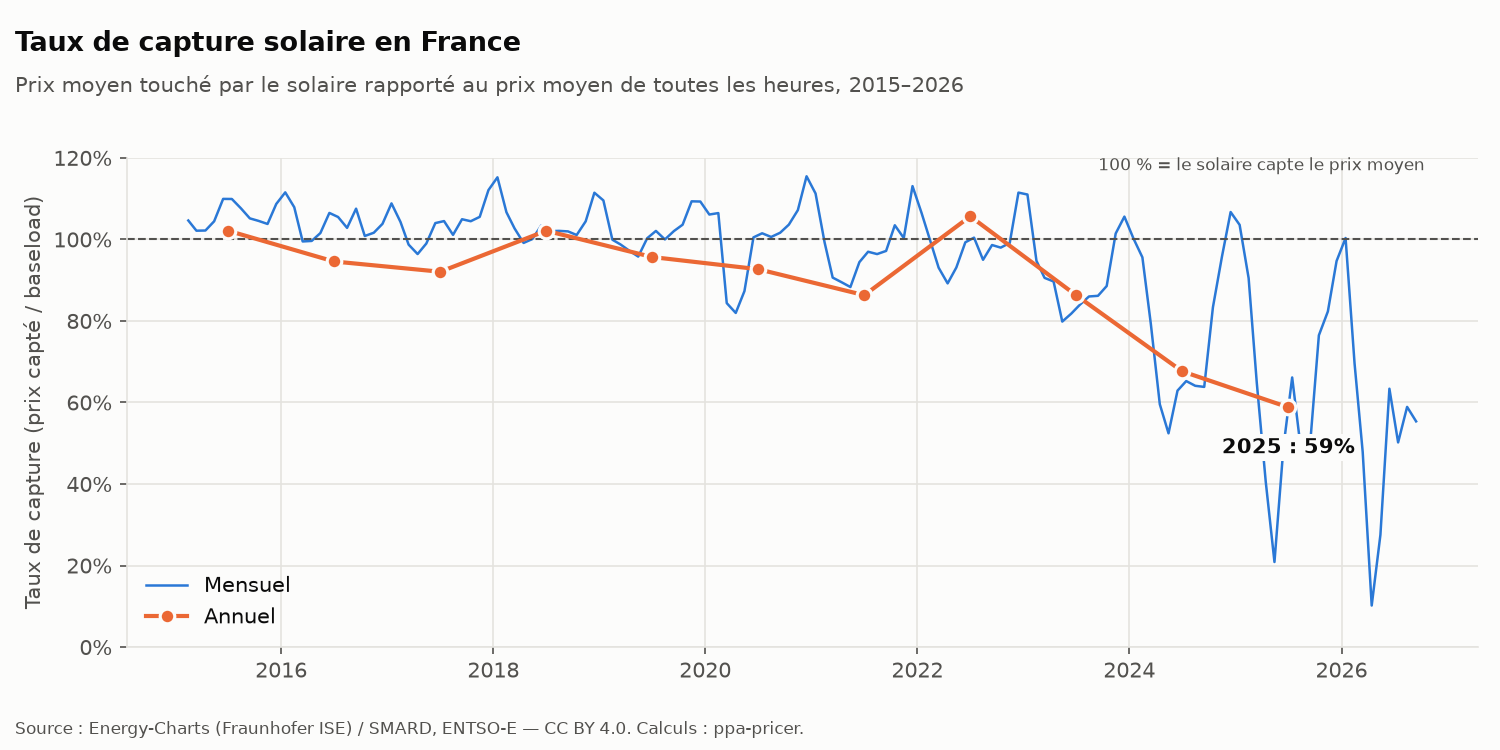
\includegraphics[width=0.9\linewidth]{taux_capture_temps.png}
\caption{Taux de capture dans le temps.}
\end{figure}

\begin{figure}[!ht]
\centering
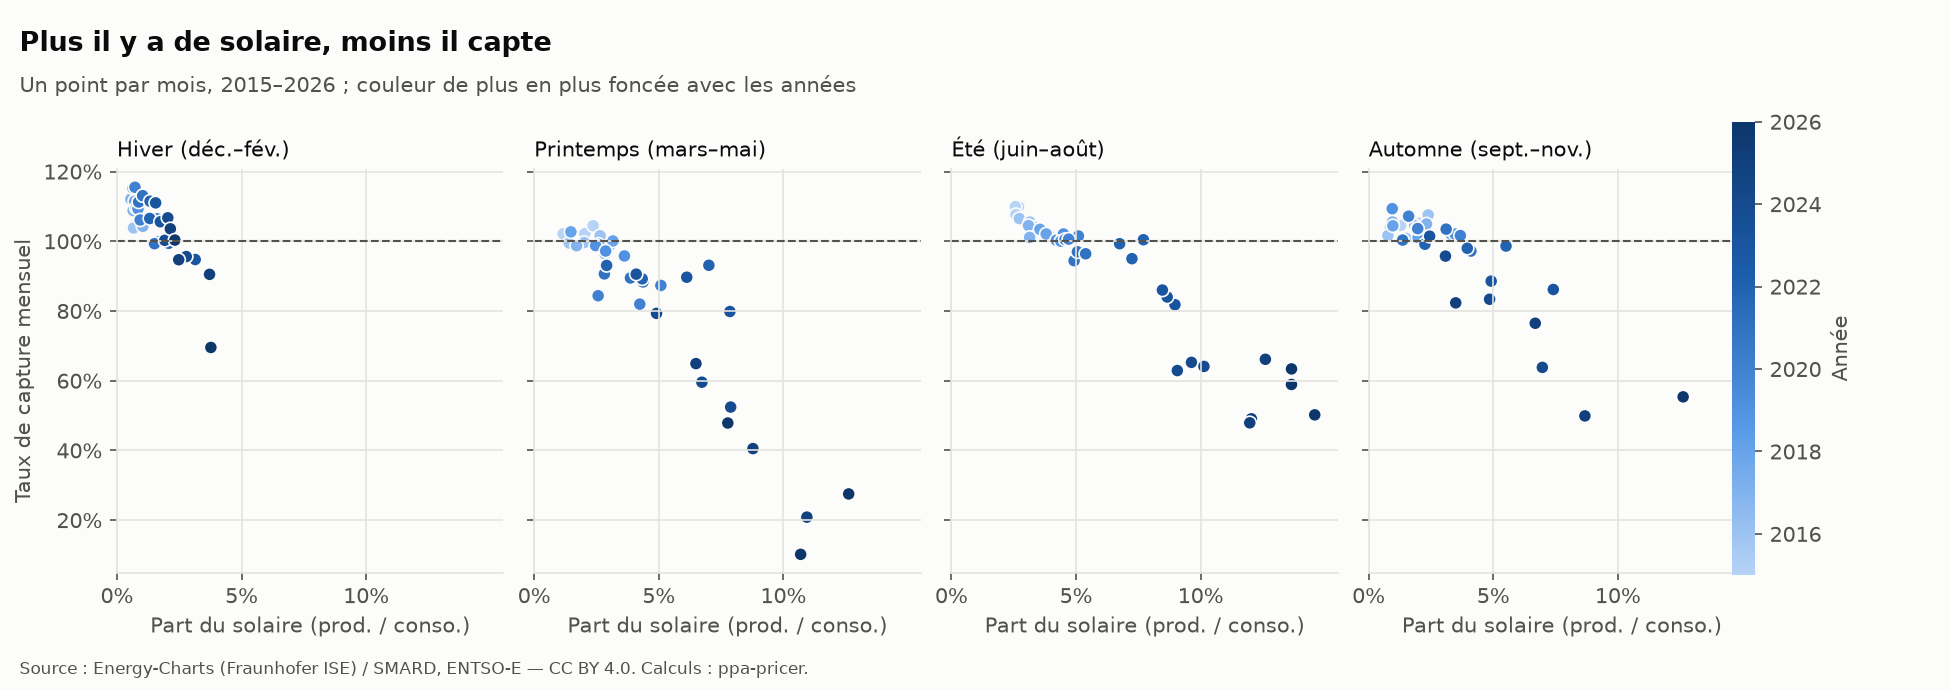
\includegraphics[width=0.9\linewidth]{part_solaire_vs_taux_capture.png}
\caption{Part du solaire et taux de capture, par saison.}
\end{figure}

\begin{figure}[!ht]
\centering
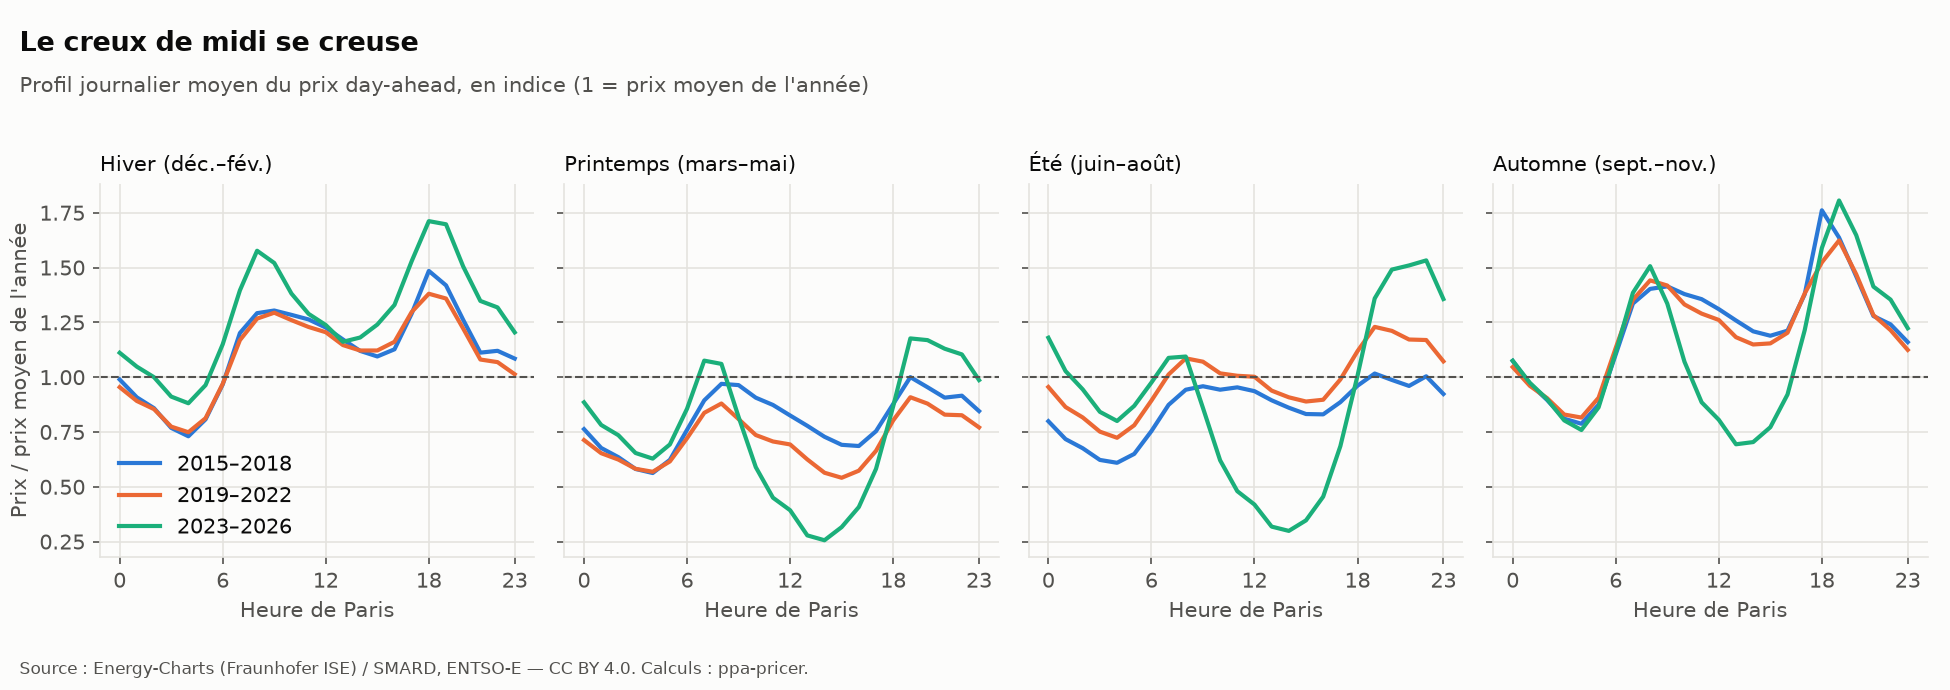
\includegraphics[width=0.9\linewidth]{profil_horaire_prix.png}
\caption{Profil horaire des prix, rapporté au prix moyen de l'année.}
\end{figure}

\begin{figure}[!ht]
\centering
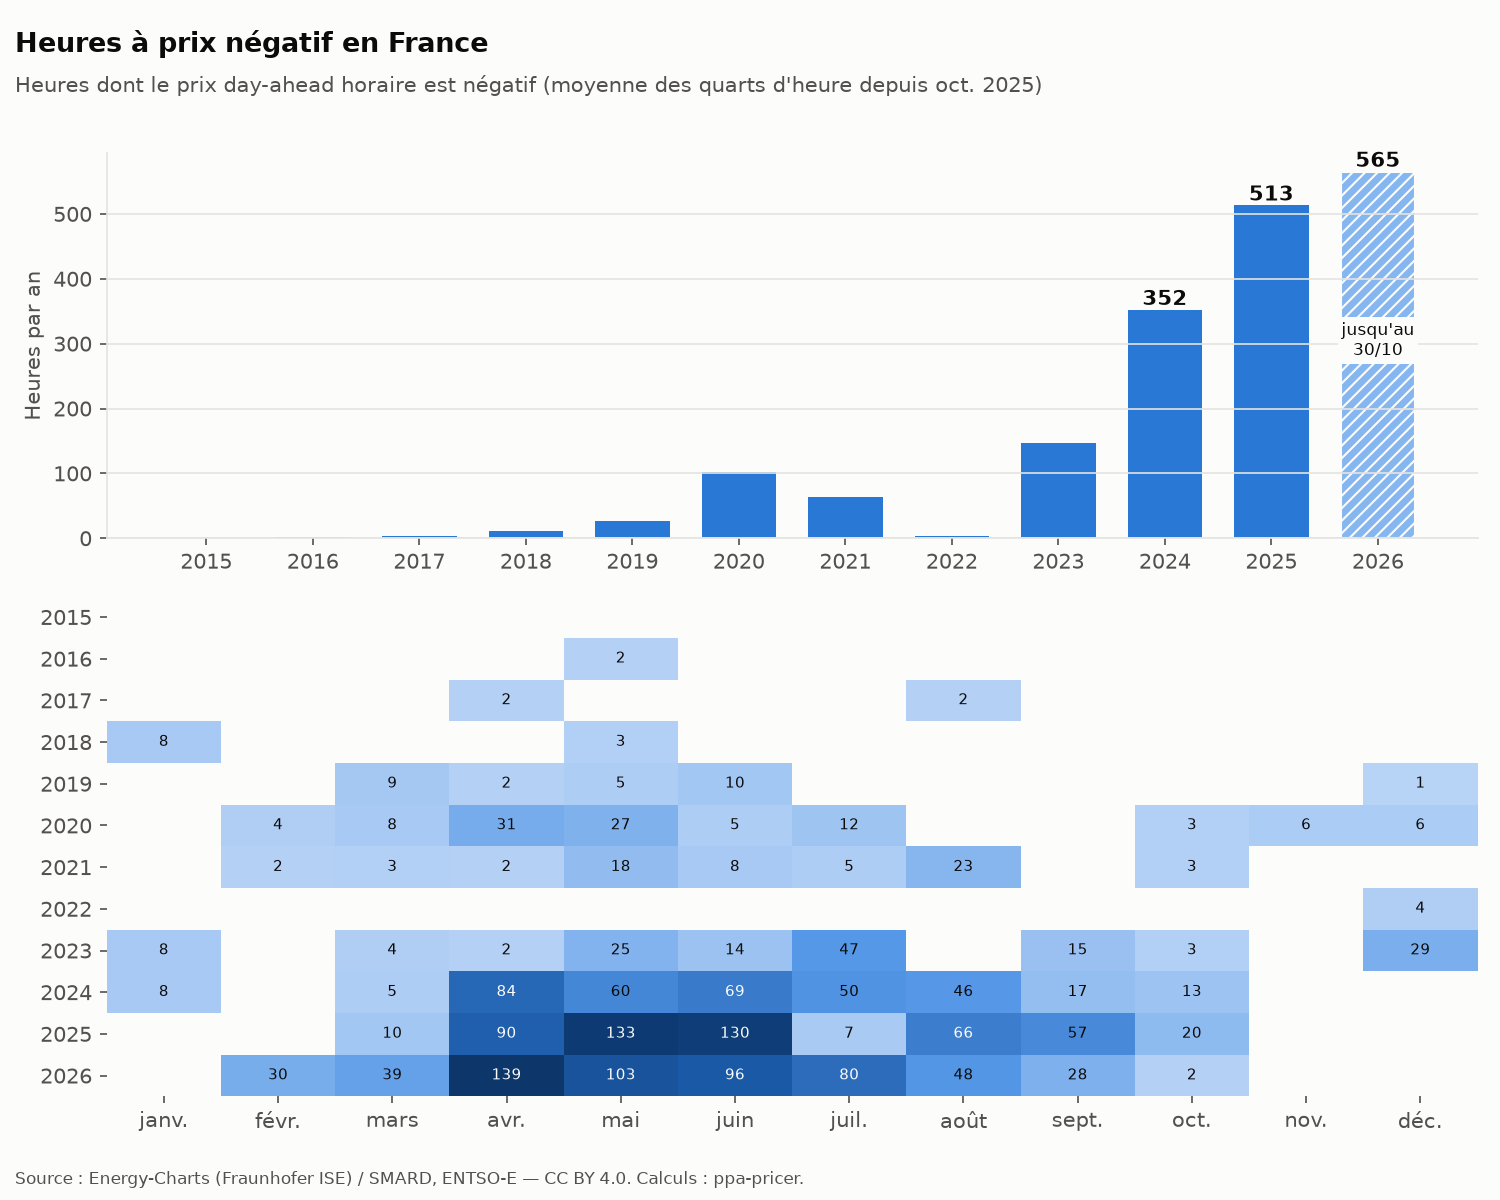
\includegraphics[width=0.9\linewidth]{heures_prix_negatifs.png}
\caption{Heures à prix négatif par année.}
\end{figure}

% ====================================================================
\section{La chaîne de données}

\begin{figure}[H]
\centering
\begin{tikzpicture}[font=\footnotesize,node distance=0.45cm,
  boite/.style={draw=bleu!70!black,fill=bleu!6,rounded corners=2pt,minimum height=0.9cm,text width=2.45cm,align=center},
  fleche/.style={-{Latex},thick,gris}]
  \node[boite] (api) {API\\Energy-Charts};
  \node[boite,right=of api] (json) {JSON brut\\par année};
  \node[boite,right=of json] (base) {SQLite\\résolution d'origine};
  \node[boite,right=of base] (ctrl) {Contrôles\\qualité};
  \node[boite,below=0.7cm of api] (hor) {Série horaire\\NaN conservés};
  \node[boite,right=of hor] (men) {Grandeurs\\mensuelles};
  \node[boite,right=of men] (mod) {Modèle V1\\par année};
  \node[boite,right=of mod] (bt) {Backtest\\et rapport};
  \draw[fleche] (api) -- (json);
  \draw[fleche] (json) -- (base);
  \draw[fleche] (base) -- (ctrl);
  \draw[fleche] (base.south) -- ++(0,-0.3) -| (hor.north);
  \draw[fleche] (hor) -- (men);
  \draw[fleche] (men) -- (mod);
  \draw[fleche] (mod) -- (bt);
\end{tikzpicture}
\caption{De la source au rapport.}
\end{figure}

\subsection{Les sources}

\begin{itemize}
\item \textbf{Prix day-ahead} : Energy-Charts (Fraunhofer ISE), qui redistribue SMARD, sous licence CC BY 4.0. Sans jeton,
d'où un démarrage simple. ENTSO-E a servi de contrôle : prix identiques sur toutes les heures communes.
\item \textbf{Production solaire et consommation} : Energy-Charts (données ENTSO-E, fournies par RTE). RTE éCO2mix sert de
point de comparaison (section~\ref{sec:calage}).
\item \textbf{Volume} : 132\,146 points de prix du 01/01/2015 au 30/10/2026, dont 95 sans valeur (1\textsuperscript{er} au 4 janvier 2015).
\end{itemize}

\subsection{Le temps : UTC en interne}

Toutes les données restent en UTC ; seules l'affectation à un mois et l'affichage utilisent Europe/Paris. En heure locale, une
journée dure 23~h au printemps, 25~h à l'automne : on aurait des heures perdues ou en double. L'API fournit des secondes Unix, sans ambiguïté.

Pandas connaît le calendrier des changements d'heure. On en déduit le nombre d'heures attendu d'un jour en localisant ses deux minuits à Paris :
\begin{codepy}
debut = pd.DatetimeIndex(pd.to_datetime(jours)).tz_localize(FUSEAU_AFFICHAGE)
fin = (pd.DatetimeIndex(pd.to_datetime(jours)) + pd.Timedelta("1D")).tz_localize(FUSEAU_AFFICHAGE)
return pd.Series(((fin - debut) / pd.Timedelta("1h")).astype(int), index=jours)
\end{codepy}

\subsection{Le passage au quart d'heure}

Les prix passent à 15~minutes le 30/09/2025 à 22~h UTC (H1), la production le 31/12/2025 à 23~h UTC (H6). La V1 reste horaire : la
valeur d'une heure est la moyenne de ses 4 quarts d'heure, et NaN si l'un manque. Pour un prix, c'est celui d'un produit à puissance constante sur l'heure.
Pour une puissance, c'est la puissance moyenne de l'heure, égale à l'énergie en MWh. La durée d'un point est déduite de la date, et non de l'écart avec le
point suivant : sinon un trou ferait croire à un point de 2~h.

\begin{codepy}
heure = serie["ts_utc"].dt.floor("h")
groupes = serie.groupby(heure)[colonnes]
attendu = serie.groupby(heure)["duree_min"].first().map({60: 1, 15: 4})
complet = groupes.count().eq(attendu, axis=0)
horaire = groupes.mean().where(complet)
grille = pd.date_range(horaire.index.min(), horaire.index.max(), freq="h", name="ts_utc")
return horaire.reindex(grille).reset_index()
\end{codepy}

\begin{attention}
\textbf{Inconnu n'est pas zéro.} Une donnée absente reste NaN. Remplacer un prix manquant par 0 ferait baisser le baseload. À l'inverse,
un solaire à 0 la nuit est un vrai zéro. Dans le JSON, les manquants arrivent en \code{null}.
\end{attention}

\subsection{Le stockage SQLite}

\begin{itemize}
\item \textbf{Clé primaire} \code{(zone, ts\_utc)} : la base interdit deux lignes pour la même heure.
\item \textbf{\code{INSERT OR REPLACE}} : relancer le chargement donne le même résultat. Le chargement est \emph{idempotent}.
\item \textbf{Dates en texte ISO} (\code{2024-06-30T10:00:00Z}) : l'ordre alphabétique est l'ordre chronologique.
\item \textbf{NaN $\leftrightarrow$ NULL} : l'inconnu survit à l'aller-retour, ce qu'un test vérifie.
\item \textbf{Transaction} (\code{with con:}) : tout est écrit, ou rien.
\item \textbf{Résolution d'origine} : l'agrégation est un choix de modèle, faite à la lecture, donc modifiable sans re-télécharger.
\item \textbf{Requêtes paramétrées} : les valeurs passent par des \code{?}, et les noms de table viennent d'un dictionnaire interne.
\end{itemize}

\subsection{Les contrôles qualité}

Principe : \textbf{compter les anomalies, ne jamais les corriger en silence}.

\begin{center}
\begin{tabularx}{\linewidth}{lYY}
\toprule
\textbf{Contrôle} & \textbf{Méthode} & \textbf{Ce qu'il attrape} \\
\midrule
Doublons & \code{ts.duplicated()} & Deux points à la même heure \\
Mal alignés & Secondes modulo la durée $\neq 0$ & Un point horaire à 14~h~30 \\
Trous & Grille attendue moins horodatages présents & Heures absentes de la source \\
Valeurs manquantes & \code{isna()} & Points présents sans valeur \\
Changements d'heure & Heures par jour de Paris contre 23, 24 ou 25 & Heure perdue ou en double \\
Calage du solaire & Heure moyenne de production et solaire de nuit & Série décalée, valeurs impossibles \\
\bottomrule
\end{tabularx}
\end{center}

\textbf{Simulation d'une erreur classique} : une source enregistre l'heure de Paris sans fuseau, et on la lit comme de l'UTC.
En automne 2024, l'heure de 2~h apparaît deux fois (1 doublon). Au printemps 2024, elle n'existe pas (1 trou, et un jour de 22~h).
Les contrôles se complètent : aucun n'attrape seul les deux cas.

\subsection{L'anomalie de calage : la meilleure histoire du projet}
\label{sec:calage}

\textbf{Le constat de départ.} Tous les contrôles de grille valent 0. Pourtant, en préparant une explication, on remarque 248~MW de solaire à
23~h, heure de Paris, en moyenne sur juin 2025 : physiquement impossible.

\textbf{Le test.} Le midi solaire ne bouge pas d'une année à l'autre. L'heure moyenne de production, pondérée par l'énergie et exprimée en UTC, doit
donc rester stable d'une année sur l'autre pour un même mois :
\[
\bar h_m = \frac{\sum_{t \in m} h_t\, e_t}{\sum_{t \in m} e_t},
\qquad
\text{écart}_m = \bar h_m - \text{médiane}\big(\bar h_{\text{même mois, toutes années}}\big),
\]
avec $h_t$ le milieu de la période et $e_t$ son énergie.

\begin{center}
\begin{tabularx}{\linewidth}{lrY}
\toprule
\textbf{Période} & \textbf{Écart} & \textbf{Lecture} \\
\midrule
2015--2022 & au plus 0,12~h & Stable : sert à situer le seuil de 0,2~h \\
Juillet 2023 & $+0{,}21$~h & Décalage visible surtout sur une semaine \\
Sept. 2023 -- mars 2024 & $+0{,}69$ à $+0{,}95$~h & Environ 1~h trop tard, retour net en avril 2024 ; déjà dans ENTSO-E \\
Janv. -- déc. 2025 & $+0{,}26$ à $+0{,}42$~h & Energy-Charts garde le premier quart d'heure \\
\bottomrule
\end{tabularx}
\end{center}

S'y ajoute du solaire de nuit, entre 21~h et 03~h UTC, à plus de 0,1\,\% de l'énergie du mois sur 13~mois (juillet--août 2018 et 2019,
juillet--septembre 2020, juin--juillet 2023, 2025 et 2026). Par exemple, 234~MW constants en pleine nuit début juin 2023.

\textbf{Effet sur les résultats}, en rejouant tout le backtest avec le solaire de RTE (ODRÉ) :

\begin{center}
\begin{tabular}{lrr}
\toprule
 & \textbf{Energy-Charts (officiel)} & \textbf{Solaire RTE (test)} \\
\midrule
Taux de capture 2023 & 86,29\,\% & 84,57\,\% \\
Taux de capture 2024 & 67,65\,\% & 64,84\,\% \\
Taux de capture 2025 & 58,81\,\% & 56,04\,\% \\
MAE du modèle réaliste, 2018--2025 & 5,95 & 5,95 \\
Skill contre R1 / contre R2 & $+0{,}10$ / $+0{,}47$ & $+0{,}12$ / $+0{,}48$ \\
p-value Diebold-Mariano contre R1 & 0,449 & 0,284 \\
\bottomrule
\end{tabular}
\end{center}

Le verdict tient, mais le taux de capture 2025 perd 2,8~points, soit environ 1,7~€/MWh.

\textbf{Le contrôle ENTSO-E a trouvé deux causes.} Ma règle, écrite avant, supposait une seule origine : 8~mois signalés sur 20 sont proches d'ENTSO-E, donc le décalage « apparaît après ENTSO-E ». C'est trop court :
\begin{itemize}
\item \textbf{2025 : Energy-Charts.} ENTSO-E passe au quart d'heure fin 2024, mais les fichiers Energy-Charts restent horaires. Sur 2025, 100\,\% de leurs valeurs égalent le \emph{premier quart d'heure} de l'heure, contre 39\,\% pour la moyenne. Une telle valeur est centrée sur $h + 7{,}5$~min au lieu de $h + 30$~min, d'où les 0,375~h d'écart apparent. L'effet réel est faible : $+0{,}25$~point sur le taux 2025.
\item \textbf{2023--2024 : ENTSO-E ou en amont.} Energy-Charts et ENTSO-E y sont identiques, et RTE s'en écarte. D'octobre à décembre 2023, la corrélation avec RTE passe de 0,95--0,96 à 0,99 avec 1~h de retard. La production de nuit vient aussi d'ENTSO-E ou d'en amont.
\end{itemize}
Les prix sont identiques entre Energy-Charts et ENTSO-E, y compris les niveaux élevés d'août à octobre 2026.

\textbf{Ce qui reste inconnu} :
\begin{itemize}
\item La cause de l'écart avec RTE : Energy-Charts vaut de 0,89 à 1,00 fois RTE selon les années. C'est ce qui pèse le plus : 2,8~points sur 2025, dont environ 1,1 par les niveaux mensuels et 1,7 par la forme dans le mois.
\item La fiabilité de RTE sur le calage : la moyenne de ses valeurs de :00 et :30 est centrée sur $h + 15$~min, ce qui expliquerait environ 0,25~h de son écart habituel de 0,33~h (probable, non vérifié).
\end{itemize}

\textbf{Décision.} Le contrôle signale sans corriger, et le verdict officiel reste calculé sur les données telles que publiées (H8) : changer les données après avoir
vu les résultats fausserait le protocole. Le choix de la source est reporté à la V2.

\begin{entretien}
« Tous mes contrôles de grille passaient. Un test physique simple, l'heure moyenne de production en UTC, a révélé un décalage qui atteint une heure fin 2023. En recoupant avec ENTSO-E et RTE, j'ai trouvé deux causes : une déjà dans ENTSO-E en 2023, et une chez Energy-Charts en 2025, qui garde le premier quart d'heure au lieu de la moyenne. J'ai mesuré l'effet sur mes résultats, et je n'ai pas corrigé après coup pour ne pas fausser le protocole. »
\end{entretien}

% ====================================================================
\section{Le modèle V1}

\subsection{La forme}

\begin{definition}{Modèle V1}
\[
\TC_m = \alpha_{\text{mois}(m)} + \beta\, S_m + \varepsilon_m
\]
12 constantes $\alpha$, une par mois calendaire, pour le niveau saisonnier ; une pente commune $\beta$ pour l'effet de la part du solaire.
\end{definition}

Pourquoi prévoir $\TC$ plutôt que le prix du PPA : le niveau baseload est donné par le marché à terme ou des scénarios, et on ne prétend pas mieux le prévoir que lui. Le
taux de capture porte la cannibalisation, où un modèle peut apporter quelque chose. Un PPA peut durer jusqu'à 20~ans, pour une dizaine d'années de données : un backtest honnête
n'est possible qu'à horizon court, ici un an.

\subsection{L'estimation}

En notant $y$ le vecteur des $\TC_m$, $D_k$ l'indicatrice du mois $k$ et $X = [D_1 \cdots D_{12}\ S]$, on résout par moindres carrés ordinaires :
\[
\hat\theta = \arg\min_\theta \|y - X\theta\|^2 = (X^\top X)^{-1} X^\top y .
\]
Il n'y a \textbf{pas de constante globale} : la somme des 12 indicatrices vaut 1, une constante rendrait $X$ de rang insuffisant (\emph{dummy variable trap}). Le code utilise
\code{numpy.linalg.lstsq}, numériquement plus stable que d'inverser $X^\top X$.

\begin{codepy}
x = np.column_stack([(mois == m).to_numpy(dtype=float) for m in MOIS] + [h["part_solaire"].to_numpy()])
coefficients, *_ = np.linalg.lstsq(x, h["taux_capture"].to_numpy(), rcond=None)
\end{codepy}

\textbf{Lecture de $\hat\beta$ (Frisch-Waugh-Lovell).} Régresser sur les indicatrices revient à retirer à chaque variable sa moyenne par mois calendaire :
\[
\hat\beta = \frac{\sum_m (S_m - \bar S_{\text{mois}(m)})(\TC_m - \overline{\TC}_{\text{mois}(m)})}{\sum_m (S_m - \bar S_{\text{mois}(m)})^2},
\qquad
\hat\alpha_k = \overline{\TC}_k - \hat\beta\, \bar S_k .
\]
$\hat\beta$ se lit donc \emph{à mois calendaire donné} : c'est la relation entre juin plus solaire et juin moins solaire, d'une année à l'autre. Sur la calibration 2026, cette formule et
\code{lstsq} donnent tous deux $-6{,}223$. Avec $\hat\beta = -6{,}22$, un point de part du solaire en plus retire 6,22~points de taux de capture.

\begin{center}
\small\setlength{\tabcolsep}{3.5pt}
\begin{tabular}{l*{9}{c}}
\toprule
Année prévue & 2018 & 2019 & 2020 & 2021 & 2022 & 2023 & 2024 & 2025 & 2026 \\
Mois de calibration & 35 & 47 & 59 & 71 & 83 & 95 & 107 & 119 & 131 \\
$\hat\beta$ & $-5{,}89$ & $-4{,}50$ & $-4{,}00$ & $-4{,}72$ & $-4{,}79$ & $-2{,}86$ & $-3{,}40$ & $-5{,}15$ & $-6{,}22$ \\
\bottomrule
\end{tabular}
\end{center}

La pente se creuse depuis 2023 : c'est cohérent avec une relation non linéaire que la forme linéaire ne capte pas.

\subsection{Prévoir la part du solaire (H4)}

La variante réaliste doit aussi prévoir $S$ :
\[
\hat S_{m,T} = S_{m,T-1} \times \frac{E_{T-1}}{E_{T-2}},
\]
avec $E$ la production solaire annuelle : on suppose que la croissance récente se prolonge.

\textbf{Exemple complet, juin 2026.} La part de juin 2025 vaut 12,03\,\%, et le rapport $E_{2025}/E_{2024}$ vaut 1,295 : on prévoit donc $\hat S = 15{,}58\,\%$. La calibration donne $\hat\alpha_6 = 1{,}2752$ et $\hat\beta = -6{,}2230$, d'où :
\[
\widehat{\TC} = 1{,}2752 - 6{,}2230 \times 0{,}1558 = 0{,}3055 = 30{,}6\,\%.
\]
Le réalisé est de 63,4\,\% : 33~points d'erreur dans ce sens, alors qu'en avril 2026 le modèle prévoit 41,4\,\% pour 10,2\,\% réalisés, 31~points dans l'autre. Une pente unique pour toutes
les saisons ne peut pas capter les deux.

\subsection{Les limites}

\begin{itemize}
\item \textbf{Linéarité} : l'analyse montre une relation coudée et saisonnière, mais la forme avait été figée avant : changer d'après ces graphiques serait du \emph{data snooping}.
\item \textbf{Extrapolation} : avant 2024, $S$ annuel n'a jamais dépassé environ 5\,\%. Le modèle prévoit donc hors de son domaine de calibration.
\item \textbf{Variables absentes} : hydraulique, disponibilité du nucléaire, demande, interconnexions et prix du gaz jouent aussi.
\item \textbf{Profil national} : le taux d'un site réel diffère du taux national (H2).
\item \textbf{H4 surestime en 2026} : la part prévue dépasse la part réalisée sur 8 des 9 mois valides.
\end{itemize}

% ====================================================================
\section{Le protocole de backtest}

\subsection{Le walk-forward}

Pour chaque année de test $T$ de 2018 à 2025, on calibre sur tous les mois valides \emph{strictement antérieurs} au 1\textsuperscript{er} janvier $T$, puis on prévoit les 12 mois de $T$.
On obtient 96 prévisions mensuelles. La fenêtre est \emph{expansive} : on garde tout l'historique. Les années 2015--2017 n'ont pas de test et restent dans toutes les calibrations ; la première compte 35~mois, car janvier 2015 est invalide.

\begin{figure}[ht]
\centering
\begin{tikzpicture}[x=1cm,y=0.36cm,font=\footnotesize]
  \foreach \T [count=\i] in {2018,...,2025} {
    \pgfmathsetmacro{\yy}{-\i}
    \pgfmathsetmacro{\fin}{\T-2015}
    \pgfmathsetmacro{\finb}{\T-2014}
    \fill[bleu!55] (0,\yy) rectangle (\fin,\yy+0.72);
    \fill[orange!85] (\fin,\yy) rectangle (\finb,\yy+0.72);
    \node[anchor=east] at (-0.1,\yy+0.36) {$T=\T$};
  }
  \foreach \a in {2015,2017,...,2025} {
    \pgfmathsetmacro{\xx}{\a-2015}
    \node[anchor=north,gris] at (\xx,-8.2) {\a};
    \draw[gris!50] (\xx,-8.15) -- (\xx,0.1);
  }
  \fill[bleu!55] (2.1,-10.6) rectangle (2.5,-10);
  \node[anchor=west] at (2.55,-10.3) {calibration};
  \fill[orange!85] (5,-10.6) rectangle (5.4,-10);
  \node[anchor=west] at (5.45,-10.3) {prévision};
\end{tikzpicture}
\caption{Walk-forward à fenêtre expansive. L'année 2026 suit le même schéma mais reste hors verdict.}
\end{figure}

\textbf{Pourquoi pas une validation croisée aléatoire ?} Une série temporelle a une dépendance : mélanger les mois laisserait le futur informer le passé. Un test pytest garantit l'absence de fuite :
il remplace toutes les données futures par 999 et vérifie que les prévisions ne changent pas.

\subsection{Deux variantes pour séparer les erreurs}

\begin{itemize}
\item \textbf{Réaliste} : $S$ est prévu par H4. C'est la vraie performance de l'outil, et celle du verdict.
\item \textbf{Conditionnelle} : on donne au modèle la part réalisée, ce qui est une triche volontaire sur cette seule entrée. Elle teste la relation $S \to \TC$ seule.
\end{itemize}

\subsection{Les références à battre}

\begin{itemize}
\item \textbf{R1, persistance} : $\widehat{\TC}_m(T) = \TC_m(T-1)$, le même mois de l'année précédente.
\item \textbf{R2, climatologie} : la moyenne de ce mois calendaire sur toutes les années antérieures.
\end{itemize}

Elles n'ont aucun paramètre estimé, comme le portefeuille $1/N$ sur les actions : un modèle qui ne les bat pas n'apporte rien.

\begin{attention}
R1 et R2 ne représentent pas le marché ni les autres acteurs. Le projet ne compare à aucune cotation réelle ni à aucune prévision professionnelle : il ne dit donc rien sur la capacité à « battre le marché ».
\end{attention}

\subsection{Les métriques}

Avec $e_m = \widehat{\TC}_m - \TC_m$ (positive si on surestime) :
\begin{gather*}
\MAE = \frac1n\sum_m |e_m|,
\qquad
\text{biais} = \frac1n\sum_m e_m,
\\
\MAE_{\text{pond.}} = \frac{\sum_m Q_m |e_m|}{\sum_m Q_m},
\qquad
\text{skill} = 1 - \frac{\MAE_{\text{modèle}}}{\MAE_{\text{réf.}}}.
\end{gather*}
\textbf{Critère de succès, figé à l'avance} : skill $> 0$ contre R1 \emph{et} contre R2, variante réaliste, 2018--2025. Toutes les méthodes sont jugées sur le même échantillon de mois.

\textbf{Passer du mensuel à l'annuel.} On combine les 12 prévisions avec le baseload et les volumes \emph{réalisés}, pour mesurer seulement la prévision du taux de capture :
\[
\widehat{\TC}_T = \frac{\sum_m \widehat{\TC}_m\, B_m\, Q_m}{B_T \sum_m Q_m}.
\]
Avec des prévisions parfaites, $\sum_m \TC_m B_m Q_m = \sum_m C_m Q_m = \sum_h q_h p_h$, et on retrouve exactement le taux annuel réalisé : un test le vérifie.

\subsection{Le pré-enregistrement}

Le \textbf{data snooping} consiste à essayer des variantes jusqu'à ce que l'une marche, puis à ne présenter qu'elle. Pour l'éviter, le protocole, le critère et la forme du modèle sont écrits dans
\code{docs/perimetre.md} avant le premier résultat. Toute modification est datée dans un journal, et les variantes futures seront figées puis jugées sur des mois publiés après le 29/10/2026.

\begin{attention}
L'analyse descriptive couvrait déjà les années de test avant le premier résultat du modèle : le pré-enregistrement ne vaut pas une ignorance totale. C'est écrit dans le journal, et il faut le dire.
\end{attention}

% ====================================================================
\section{Le test de Diebold-Mariano}

\subsection{La question}

Le modèle a un MAE plus faible que R1. Est-ce une vraie différence de précision, ou le hasard de ces 96~mois ?

\subsection{La construction}

\begin{enumerate}
\item Écart de perte mensuel : $d_t = |e^{A}_t| - |e^{B}_t|$. Il est négatif quand A se trompe moins que B.
\item Hypothèse nulle : $H_0 : \mathbb{E}[d_t] = 0$, même précision.
\item Statistique : $\mathrm{DM} = \bar d \,/\, \sqrt{\hat V / n}$.
\item p-value bilatérale d'une loi de Student à $n-1$ degrés de liberté, presque identique à la loi normale ici, car $n = 96$ ; le vrai petit échantillon, ce sont les 8 années, d'où le bootstrap par années de l'audit.
\end{enumerate}

Les $d_t$ ne sont pas indépendants : tous les mois d'une année utilisent la même calibration, et un écart persiste d'un mois à l'autre. On estime donc la variance de long terme par Newey-West, avec le noyau de Bartlett :
\[
\hat V = \hat\gamma_0 + 2\sum_{k=1}^{L}\Big(1 - \frac{k}{L+1}\Big)\hat\gamma_k,
\qquad
\hat\gamma_k = \frac1n\sum_{t=k+1}^{n}(d_t - \bar d)(d_{t-k} - \bar d).
\]
Les poids de Bartlett garantissent $\hat V \ge 0$. On prend $L = 11$ retards, car les prévisions d'une année forment un bloc de 12~mois.

\subsection{Pourquoi la correction compte}

Pour le modèle réaliste contre R1, $\bar d = -0{,}67$~point et l'autocorrélation d'ordre~1 de $d_t$ vaut 0,60. Ignorer cette dépendance exagère la significativité :

\begin{center}
\begin{tabular}{lccccc}
\toprule
Retards $L$ & 0 & 3 & 6 & \textbf{11} & 23 \\
Statistique DM & $-1{,}46$ & $-0{,}93$ & $-0{,}81$ & $\mathbf{-0{,}76}$ & $-0{,}81$ \\
\bottomrule
\end{tabular}
\end{center}

\subsection{Comment le lire}

\begin{itemize}
\item Contre R1 : $-0{,}76$, $p = 0{,}449$ : on ne peut pas conclure que le modèle est meilleur.
\item Contre R2 : $-2{,}76$, $p = 0{,}007$ : le modèle est significativement meilleur.
\item \textbf{Non significatif ne veut pas dire équivalent} : huit années laissent peu de puissance au test.
\item DM compare des \emph{prévisions} sur un échantillon, pas la vérité de deux modèles.
\item Il existe une correction de petit échantillon (Harvey, Leybourne et Newbold, 1997) que nous n'appliquons pas : nous gardons seulement la loi de Student.
\end{itemize}

% ====================================================================
\section{Les résultats}

\subsection{Le verdict}

Skill $+0{,}10$ contre R1 et $+0{,}47$ contre R2 : \textbf{le critère est atteint}.

\begin{center}
\begin{tabular}{lrrrrr}
\toprule
\textbf{2018--2025, 96 mois} & MAE & MAE pond. & Biais & Skill R1 & Skill R2 \\
\midrule
Modèle réaliste & 5,9 & 8,5 & 3,3 & $+0{,}10$ & $+0{,}47$ \\
Modèle conditionnel & 5,9 & 8,4 & 2,4 & $+0{,}11$ & $+0{,}47$ \\
R1 persistance & 6,6 & 8,9 & 4,8 & --- & $+0{,}41$ \\
R2 climatologie & 11,2 & 17,3 & 10,4 & $-0{,}69$ & --- \\
\bottomrule
\end{tabular}
\end{center}

\begin{center}
\begin{tabular}{lrrrr}
\toprule
\textbf{Diebold-Mariano} & Écart moyen & Statistique & p-value \\
\midrule
Réaliste contre R1 & $-0{,}7$ & $-0{,}76$ & 0,449 \\
Réaliste contre R2 & $-5{,}2$ & $-2{,}76$ & 0,007 \\
Conditionnel contre R1 & $-0{,}7$ & $-1{,}10$ & 0,273 \\
Conditionnel contre R2 & $-5{,}2$ & $-2{,}33$ & 0,022 \\
\bottomrule
\end{tabular}
\end{center}

\subsection{Par année}

\begin{center}
\begin{tabular}{lrrrr|rrr}
\toprule
 & \multicolumn{4}{c|}{\textbf{MAE mensuelle (points)}} & \multicolumn{3}{c}{\textbf{Taux annuel}} \\
\textbf{Année} & Réaliste & Condit. & R1 & R2 & Réalisé (\%) & Err.\ réaliste & Err.\ R1 \\
\midrule
2018 & 2,8 & 2,1 & 2,4 & 2,5 & 102,1 & $-1{,}2$ & $+0{,}3$ \\
2019 & 2,3 & 2,0 & 3,1 & 3,3 & 95,7 & $+0{,}1$ & $+2{,}0$ \\
2020 & 5,8 & 4,7 & 4,9 & 6,2 & 92,7 & $-0{,}9$ & $+1{,}8$ \\
2021 & 2,0 & 3,0 & 4,6 & 5,7 & 86,3 & $-0{,}4$ & $+1{,}9$ \\
2022 & 2,9 & 5,8 & 2,6 & 4,2 & 105,7 & $-3{,}0$ & $-1{,}2$ \\
2023 & 3,2 & 3,8 & 8,2 & 10,7 & 86,3 & $+2{,}0$ & $+8{,}1$ \\
2024 & \textbf{11,5} & 13,8 & 14,5 & 23,5 & 67,6 & $\mathbf{+10{,}4}$ & $+12{,}9$ \\
2025 & \textbf{17,1} & 12,2 & 12,5 & 33,0 & 58,8 & $\mathbf{+13{,}3}$ & $+9{,}3$ \\
\midrule
\textbf{MAE annuelle} & & & & & & \textbf{3,9} & \textbf{4,7} \\
\bottomrule
\end{tabular}
\end{center}

\subsection{Les autres tests}

\begin{itemize}
\item \textbf{Sans 2022} (84~mois, sensibilité à la crise des prix) : réaliste 6,4, R1 7,2, R2 12,1. Skill $+0{,}11$ et $+0{,}47$ : le verdict ne dépend pas de cette année.
\item \textbf{2026, hors verdict} (9~mois valides, janvier--septembre) : réaliste 15,7, R1 13,9, R2 39,7. \textbf{Skill $-0{,}13$ contre R1} : le modèle fait moins bien que la persistance.
\end{itemize}

\subsection{Comment l'interpréter}

\begin{enumerate}
\item \textbf{Le verdict officiel est positif, mais fragile.} L'avantage sur R1 n'est pas significatif, et il est négatif sur 2025 et 2026.
\item \textbf{Les erreurs se concentrent sur le régime récent.} MAE de 2 à 6~points jusqu'en 2023, puis de 11,5 à 17,1 en 2024--2025.
\item \textbf{Le biais est positif sur 2018--2025} : le modèle surestime le taux de capture, ce qui est cohérent avec une cannibalisation qui accélère plus vite qu'une droite.
\item \textbf{L'erreur vient surtout de la relation, pas de la prévision de $S$} : connaître la part réalisée laisse le MAE à 5,9, et aggrave même 2024 (13,8 contre 11,5). En 2025, elle aide : 12,2 contre 17,1.
\item \textbf{R2 s'effondre} parce qu'elle moyenne un passé où le solaire comptait peu : ne pas modéliser la tendance coûte cher.
\end{enumerate}

\begin{entretien}
« Le critère figé à l'avance est atteint, mais je ne m'en servirais pas tel quel pour pricer. Contre la persistance, l'avantage n'est pas significatif. En 2025, je surestime le taux de capture de
13~points, soit environ 8~€/MWh : 44 prévus contre 36 réalisés. Ce résultat m'a conduit à tester des formes non linéaires et des prix horaires : aucune ne résout 2024. »
\end{entretien}

% ====================================================================
\section{Du taux de capture au prix}
\label{sec:pricing}

\begin{attention}
\textbf{Cette section décrit le pricing V1, à un baseload de 61~€/MWh.} Ce niveau vaut la moitié de la cotation 2027 : ces chiffres montrent la méthode, pas le prix 2027. Le prix de référence, environ 71~€/MWh, est celui de la V2 (section~\ref{sec:v2}).

\medskip
Le résultat est une \textbf{valeur de l'énergie au spot}, pas un prix de contrat : ni garanties d'origine, ni coûts d'équilibrage, ni risque de crédit, ni marge. Code : \code{pricing/v1.py}, rapport : \code{reports/pricing/v1/rapport.md}, décisions : \code{docs/pricing.md}.
\end{attention}

\subsection{La formule}

Pour un PPA pay-as-produced d'un an, avec $V_m$ le volume mensuel du site et $B_m$ le baseload du mois dans un scénario :
\[
\text{prix juste} = \frac{\sum_m B_m\;\widehat{\TC}_m\;V_m}{\sum_m V_m}.
\]

\subsection{Les entrées, pour une livraison en 2027}

\begin{itemize}
\item \textbf{Taux de capture} : modèle V1 (140~mois de calibration, $\hat\beta = -6{,}16$) et persistance (même mois dans les 12 derniers mois valides), côte à côte.
\item \textbf{Part du solaire (H9)} : H4 demande une année 2026 complète et renvoie NaN. On prend donc les 12 derniers mois valides, d'octobre 2025 à septembre 2026, multipliés par leur croissance sur 12~mois ($+20{,}8\,\%$). Sur une année civile, cette version donne exactement H4.
\item \textbf{Baseload (H5)} : 50 / 61 / 77~€/MWh, soit les niveaux observés en 2018, en 2025 et sur les 12 derniers mois. La forme mensuelle est la moyenne 2024--2025, renormalisée pour que le niveau annuel du scénario reste exact.
\item \textbf{Volumes (H10)} : PVGIS à Montpellier, 1~MWc, plein sud, inclinaison optimale de 39°, pertes de 14\,\%, moyenne de chaque mois sur 2005--2023, soit 1\,500~MWh/MWc par an.
\end{itemize}

\subsection{Les résultats}

\begin{center}
\small
\begin{tabular}{lrrrrr}
\toprule
\textbf{Scénario} & Baseload & Modèle & Taux implicite & Persistance & Taux implicite \\
\midrule
Bas & 50 & 26,5 & 53,1\,\% & 30,4 & 60,8\,\% \\
\textbf{Central} & \textbf{61} & \textbf{32,4} & 53,1\,\% & \textbf{37,1} & 60,8\,\% \\
Haut & 77 & 40,9 & 53,1\,\% & 46,8 & 60,8\,\% \\
\bottomrule
\end{tabular}
\end{center}

Prix et baseload en €/MWh. Le revenu central vaut environ 48\,500~€/MWc par an avec le modèle et 55\,600~€/MWc avec la persistance. L'écart de 4,7~€/MWh entre les deux est du même ordre que les erreurs passées, qui valent 6,3 et 8,1~€/MWh pour le modèle sur 2024--2025 à ce baseload et à forme réalisée. À forme connue d'avance, l'erreur moyenne sur 2018--2025 est de 5,9~points, et de 13,8 au pire.

\subsection{Les sensibilités}

$\mathrm{d}K = \TC\,\mathrm{d}B + B\,\mathrm{d}\TC$. À $B \approx 61$~€/MWh, un point de taux de capture vaut environ 0,6~€/MWh. Le prix est aussi très sensible à la croissance du solaire :

\begin{center}
\small
\begin{tabular}{lccccc}
\toprule
Croissance appliquée & $+0\,\%$ & $+10\,\%$ & $+20\,\%$ & $+30\,\%$ & $+40\,\%$ \\
Prix du modèle, scénario central (€/MWh) & 38,4 & 35,5 & 32,6 & 29,7 & 26,7 \\
\bottomrule
\end{tabular}
\end{center}

\subsection{L'effet du profil du site}

Avec les volumes nationaux à la place de ceux du site, le prix central tomberait à 24,8~€/MWh pour le modèle et 31,2~€/MWh pour la persistance. Ce site produit plus en hiver que le parc national : janvier pèse 6,3\,\% de son volume, contre 3,1\,\% au national. Or c'est en hiver que le baseload et le taux de capture sont élevés.

\subsection{Mesurer l'erreur de H2}

H2 suppose que le taux de capture d'un mois est le même pour le site et pour le pays. Sur chaque année complète, on compare la formule au taux réel du site, calculé avec les prix réels et la série PVGIS de l'année : \textbf{0,6~point d'écart absolu moyen sur 2016--2023}, 1,7~point au plus.

\begin{attention}
PVGIS s'arrête en 2023. Ce contrôle ne couvre pas le régime récent, où les prix varient davantage au sein d'une journée : il ne valide pas H2 pour 2027.
\end{attention}

\subsection{Exemple rétrospectif sur 2025}

On prend le baseload et les volumes nationaux réalisés, que personne ne connaissait à l'avance : ce n'est donc pas un prix qu'on aurait pu afficher début 2025. Il mesure seulement l'effet de l'erreur sur le taux de capture.

\begin{center}
\begin{tabular}{lrr}
\toprule
\textbf{Méthode} & \textbf{Prix (€/MWh)} & \textbf{Écart au réalisé} \\
\midrule
Réalisé (prix capté) & 35,9 & --- \\
R1 persistance & 41,6 & $+5{,}7$ \\
Modèle réaliste & 44,0 & $+8{,}1$ (soit $+23\,\%$) \\
\bottomrule
\end{tabular}
\end{center}

\subsection{Ce qui manque pour un vrai prix}

La durée du contrat et l'actualisation, les garanties d'origine, les coûts d'équilibrage, le risque de crédit, la marge, l'arrêt réel aux prix négatifs (H3), et un taux de capture propre au site sur le régime récent. La courbe à terme est intégrée par la V2.

% ====================================================================
\section{Modèle stochastique, risques et pricing V2}

\begin{attention}
M0, M1, M2, un Monte-Carlo sur un an et le pricing V2, présentés ci-dessous, sont codés, ainsi qu'une appli Streamlit privée qui les reprend. Les contrats pluriannuels ne le sont pas : à présenter comme une direction, jamais comme un résultat.
\end{attention}

\subsection{Le processus d'Ornstein-Uhlenbeck}

Le prix de l'électricité revient vers un niveau moyen, contrairement à une action : c'est ce que capture ce processus.
\[
\mathrm{d}X_t = \kappa\,(\mu - X_t)\,\mathrm{d}t + \sigma\,\mathrm{d}W_t .
\]
$\kappa$ est la vitesse de rappel, $\mu$ le niveau long terme, $\sigma$ la volatilité. La solution est :
\[
X_t = \mu + (X_0 - \mu)\,e^{-\kappa t} + \sigma\int_0^t e^{-\kappa (t-s)}\,\mathrm{d}W_s ,
\]
d'où $\mathbb{E}[X_t] = \mu + (X_0 - \mu)e^{-\kappa t}$ et $\mathrm{Var}[X_t] = \frac{\sigma^2}{2\kappa}\big(1 - e^{-2\kappa t}\big)$. La variance stationnaire vaut $\sigma^2/(2\kappa)$ et la demi-vie d'un écart vaut $\ln 2 / \kappa$.

\textbf{Estimation.} La discrétisation exacte au pas $\Delta$ est un AR(1) :
\[
X_{t+\Delta} = \mu(1-\varphi) + \varphi X_t + \eta_t,
\qquad \varphi = e^{-\kappa\Delta},
\qquad \eta_t \sim \mathcal N\Big(0,\ \tfrac{\sigma^2}{2\kappa}(1-\varphi^2)\Big).
\]
Il suffit de régresser $X_{t+\Delta}$ sur $X_t$, puis $\hat\kappa = -\ln\hat\varphi / \Delta$.

\textbf{Limites pour l'électricité} : pas de sauts, pas de saisonnalité, et un modèle sur le log des prix est impossible avec des prix négatifs. Il faudrait ajouter une composante saisonnière déterministe, des sauts, et conditionner le prix à la production solaire nationale, avec la croissance du parc en paramètre.

\subsection{Le premier test : M0}

M0 applique ce processus au prix rapporté au baseload de son année, avec $x_t$ un AR(1) gaussien, calibré sur les deux années précédentes :
\[
y_t = s(\text{mois}, \text{heure}, \text{week-end}) + x_t .
\]
 C'est une référence \emph{sans verdict} (\code{modele/m0.py}, \code{docs/stochastique.md}). Les attentes ont été écrites avant le premier résultat.

\begin{center}
\small
\begin{tabular}{lcc}
\toprule
\textbf{Mesure} & \textbf{M0 simulé} & \textbf{Réel} \\
\midrule
Autocorrélation à 24~h (2025) & 0,26 & 0,55 \\
Autocorrélation à 48~h (2025) & 0,05 & 0,31 \\
Kurtosis du résidu (2025) & 2,96 & 5,75 \\
Prix médian à midi, avril--août 2025 (part du baseload) & 0,45 & 0,00 \\
\bottomrule
\end{tabular}
\end{center}

\begin{itemize}
\item \textbf{Intervalle à 90\,\%} : il ne contient que 41,7\,\% des taux de capture réalisés sur 2018--2025, et 16,7\,\% en 2024 comme en 2025.
\item \textbf{Précision} : MAE de 8,1 contre 6,6 pour la persistance et 5,9 pour la V1. J'attendais un résultat proche de la persistance : c'était faux, car une fenêtre de deux ans retarde quand le taux de capture baisse.
\item \textbf{Fragilité de l'estimation} : pour 2018, $\hat\varphi = 0{,}636$ au lieu d'environ 0,95. Six heures, dont trois à 874, 850 et 830~€/MWh en novembre 2016, font 46\,\% de la somme des résidus au carré.
\end{itemize}

La suite doit donc apporter deux vitesses, des queues épaisses, des prix qui restent près de 0, et une incertitude de niveau.

\subsection{Deuxième test : M1, une loi par case et deux vitesses}

M1 garde la distribution réelle des prix de chaque case. Il remplace chaque prix par son score normal, $z_t = \Phi^{-1}\big((r_t - 0{,}5)/n\big)$, avec $r_t$ son rang dans la case. Ce score suit deux Ornstein-Uhlenbeck indépendants, l'un rapide et l'autre lent :
\[
z_t = \sqrt{w}\,a_t + \sqrt{1-w}\,b_t ,
\qquad
y_t = F^{-1}_{\text{case}}\big(\Phi(z_t)\big).
\]
C'est une \textbf{copule gaussienne} : la dépendance dans le temps est gaussienne, pas la loi des prix. Les rangs rendent l'estimation insensible à la taille des pics. Aucune demi-vie aberrante : de 2,5 à 5,4~h et de 45 à 157~h.

\begin{center}
\small
\begin{tabular}{lccc}
\toprule
\textbf{Mesure} & \textbf{M1} & \textbf{M0} & \textbf{Réel} \\
\midrule
Autocorrélation à 24~h (2025) & 0,36 & 0,26 & 0,55 \\
Autocorrélation à 48~h (2025) & 0,25 & 0,05 & 0,31 \\
Kurtosis du résidu (2025) & 4,36 & 2,96 & 5,75 \\
Kurtosis du résidu (2019) & 10,78 & 3,03 & 5,75 \\
Couverture de l'intervalle à 90\,\%, taux de capture & 35,4\,\% & 41,7\,\% & --- \\
Couverture de l'intervalle à 90\,\%, baseload du mois & 45,8\,\% & 29,2\,\% & --- \\
\bottomrule
\end{tabular}
\end{center}

\begin{attention}
\textbf{Le critère du protocole n'est pas atteint} (skill de $-0{,}23$ contre R1), comme attendu. Mais j'attendais une meilleure couverture du taux de capture : c'était faux. Depuis 2020, M0 et M1 couvrent tous deux 31,9\,\% des mois. Le taux de capture d'un même mois varie en moyenne absolue de 6,6~points d'une année à l'autre, et la demi-largeur de l'intervalle à 90\,\% n'est que de 4,2~points : ces modèles simulent le bruit à l'intérieur d'une année, pas le changement de profil entre les années.
\end{attention}

\subsection{Troisième test : M2, le rang conditionné à la charge résiduelle}

M2 relie enfin le prix au parc solaire. La charge résiduelle $R_t = \text{conso}_t - \text{solaire}_t - \text{éolien}_t$, réduite dans sa case en $x_t$, agit sur le rang du prix :
\[
z_t = \lambda\, x_t + \sqrt{1-\lambda^2}\;\varepsilon_t ,
\qquad
y_t = F^{-1}_{\text{case}}\big(\Phi(z_t)\big),
\]
où $\varepsilon_t$ suit les deux Ornstein-Uhlenbeck de M1. Avec $\lambda = 0$, on retrouve M1. Plus de solaire baisse $R_t$, donc le rang, et le prix reste dans les valeurs observées de la case : une première version, additive, n'avait aucun plancher et donnait un taux de capture de 2,7\,\%. Chaque trajectoire tire la météo par semaines dans la fenêtre et une croissance du parc parmi celles déjà observées. $\lambda$ reste entre 0,48 et 0,63. En calibration, l'effet de $+10\,\%$ de solaire passe seul de $-0{,}8$ à $-5{,}4$~points entre 2018--2019 et 2024--2025 : c'est le coude de la cannibalisation, sans forme imposée.

\begin{center}
\small
\begin{tabular}{lccccc}
\toprule
\textbf{Période} & \textbf{MAE M2} & \textbf{MAE V1} & \textbf{MAE R1} & \textbf{Couverture M2} & \textbf{Largeur M2} \\
\midrule
2018--2023 & 3,3 & 3,2 & 4,3 & 76,4\,\% & 9,8 \\
2024--2025 & 13,9 & 14,3 & 13,5 & 37,5\,\% & 16,9 \\
2026 (9 mois, à part) & 15,7 & 15,7 & 13,9 & 44,4\,\% & 32,0 \\
\bottomrule
\end{tabular}
\end{center}

\begin{attention}
\textbf{Le critère n'est pas atteint} : couverture de 66,7\,\%, au lieu de 85 à 95\,\%. Le skill est de $+0{,}10$ contre R1 ($p = 0{,}105$) et de $+0{,}002$ contre la V1 ($p = 0{,}985$) : c'est une égalité. M2 bat nettement M1 ($p = 0{,}004$). Pour 2027, à définition égale, M2 donne 30,0~€/MWh, contre 32,4 pour la V1 et 37,1 pour la persistance. Son niveau reste à prendre avec prudence : sur 2026, avec la bonne croissance, le modèle est 6,3~points trop bas.
\end{attention}

\begin{aretenir}
\textbf{Le test le plus instructif} : même avec la vraie charge résiduelle française de 2024, heure par heure, le modèle reste 15,5~points trop haut. La chute de 2024 ne vient donc pas de la prévision du solaire français, du moins à travers la forme de M2.
\end{aretenir}

\textbf{Et le nucléaire, l'hydraulique, les voisins ?} Je les ai testés avec une règle écrite avant le test, mais après avoir vu le biais de $+15{,}5$~points : une variable explique 2024 si le biais passe sous 5~points. Aucune variante ne réussit : le biais reste entre $+14{,}5$ et $+15{,}5$~points. Cela ne les met pas hors de cause. D'avril à août 2024, le prix réel vaut 0,23 fois le baseload à midi et 0,82 aux autres heures (ratio 0,29). Avec le nucléaire et l'hydraulique, le modèle donne 0,54 et 0,81 (ratio 0,67) : il baisse toutes les heures presque autant. Or le taux de capture est un ratio. J'ai donc testé un $\lambda$ par heure et par saison, soit 48 coefficients : le ratio descend à 0,54, mais le biais reste à $+12{,}0$~points. \textbf{La cause de la chute de 2024 reste non établie.} Sept essais ont visé cette année : j'arrête là, car seuls des mois nouveaux pourront trancher.


\subsection{Monte-Carlo : le revenu d'un MWc en 2027, et qui porte quel risque}

Chaque trajectoire tire les prix et le solaire de M2, une année de volumes PVGIS, un baseload annuel et une erreur de modèle. Le baseload suit une loi lognormale de moyenne 61~€/MWh, de $\sigma = 0{,}25$ et corrélée à 0,65 au taux de capture : deux \textbf{hypothèses}, sans donnée de marché. Le prix horaire vaut $p_t = B\,y_t$. Avec $L = \mathbb{E}[X] - X$ :
\[
\mathrm{VaR}_{95}(L) = q_{95}(L),
\qquad
\mathrm{CVaR}_{95}(L) = \mathbb{E}[L \mid L \ge \mathrm{VaR}_{95}(L)].
\]
Chaque contrat répartit le revenu au spot $R = \sum_t q_t p_t$ : vendeur + acheteur $= R$, et le prix juste annule l'espérance de l'acheteur.

\begin{center}
\small
\begin{tabular}{lllcc}
\toprule
\textbf{Contrat} & \textbf{Côté} & \textbf{Prix (€/MWh)} & \textbf{VaR 95\,\% (€/MWc)} & \textbf{Corr. baseload} \\
\midrule
Spot, sans contrat & vendeur & --- & 23\,300 & $+0{,}94$ \\
Pay-as-produced & vendeur & 31,4 & 2\,900 & $+0{,}17$ \\
Pay-as-produced & acheteur & 31,4 & 23\,000 & $+0{,}94$ \\
Plancher à 20~€/MWh & vendeur & prime de 13,7 & 21\,600 & $+0{,}95$ \\
Plancher à 20~€/MWh & acheteur & prime de 13,7 & 4\,200 & $+0{,}21$ \\
Ruban & vendeur & 60,9 & 17\,200 & $-0{,}81$ \\
Ruban & acheteur & 60,9 & 33\,800 & $+1{,}00$ \\
\bottomrule
\end{tabular}
\end{center}

Ces chiffres supposent un baseload de 61~€/MWh, soit la moitié de la cotation 2027 : la section suivante refait le calcul sur la courbe. À baseload égal, M2 donne 31,0~€/MWh, contre 32,4 pour la V1 et 37,1 pour la persistance. Attribuée par covariance, la variance de $\ln R = \ln Q + \ln B + \ln TC$ vient à environ 72\,\% du baseload, 26\,\% du taux de capture et 2\,\% du volume.

\begin{aretenir}
\textbf{Le ruban surcouvre le producteur solaire.} Il a vendu 1\,500~MWh au baseload, mais sa production n'en capte qu'environ la moitié : il perd quand les prix montent. \textbf{Un plancher horaire transfère peu de risque annuel} : à 20~€/MWh, sa prime, rendue en espérance, ne réduit la VaR que de 9\,\% en moyenne sur 10 graines, car le put paie presque chaque jour d'été. Ces primes restent peu fiables : le modèle simule trop d'heures négatives, et trop profondes.
\end{aretenir}

\begin{attention}
\textbf{Cette VaR est trop faible.} Le taux de capture annuel réalisé ne tombe dans l'intervalle à 90\,\% que 2 années sur 8 au national et 3 sur 8 au site, et le baseload sort de son intervalle 4 années sur 10, pour 1 attendue. Avec l'erreur mesurée au site, la VaR passe de 22\,600 à 24\,000~€ ; avec les variations historiques du baseload, crise comprise, à 33\,800~€. Ces constats viennent après le résultat, et l'horizon reste d'un an.
\end{attention}

\subsection{Pricing V2 : ancrer le prix sur la courbe à terme}
\label{sec:v2}

Le baseload de 61~€/MWh vaut la moitié de la cotation. La V2 change deux choses. \textbf{Le niveau} vient de la clôture du 29/10/2026, relevée sur Selectra, qui cite EEX : CAL~27 à 122,61~€/MWh, T1 à T4 à 194,38 ; 80,61 ; 96,09 ; 120,50~€/MWh. \textbf{Le taux de capture} dépend de la part du solaire et du niveau du trimestre :
\[
TC_m = \alpha_{\text{mois}} + \beta\, S_m + \gamma \ln B_q + \delta\, S_m \ln B_q .
\]
La part suit des scénarios de parc : 37,6~GW à mi-2027 au rythme de la PPE3, 40~GW au rythme récent, 42~GW si cela accélère. La part dans la production fait moins bien que la part dans la consommation (6,9 contre 5,9 d'erreur), car le retour du nucléaire la maintient à 4,5\,\% en 2023 comme en 2024.

\begin{center}
\small
\begin{tabular}{lcccc}
\toprule
\textbf{Parc à mi-2027} & \textbf{V2} & \textbf{V1, part seule} & \textbf{Persistance} & \textbf{Implicite de la courbe} \\
\midrule
37,6~GW & 74,6 & 68,1 & 74,0 & 84,0 \\
\textbf{40~GW} & \textbf{70,6} & 63,6 & 74,0 & 83,0 \\
42~GW & 67,3 & 59,9 & 74,0 & 82,2 \\
\bottomrule
\end{tabular}
\end{center}

En backtest 2018--2025, avec le niveau réalisé, V2 a 5,2 points d'erreur moyenne, contre 5,9 pour la V1 et 6,6 pour R1 ; avec le niveau de l'année précédente, 5,3. Le gain sur la V1 n'est pas significatif ($p = 0{,}314$).

\begin{attention}
\textbf{La forme de V2 a été choisie après avoir vu ces années} : ce backtest ne la valide pas, et ses paramètres sont instables. Seuls les mois publiés après le 29/10/2026 la jugeront. Le biais de 2024 reste à $+6{,}3$~points. La moitié du revenu vient de T1, pour 22\,\% du volume. Le prix suit la cotation : à CAL~28 et CAL~29, il tombe à 34,2 et 29,5~€/MWh. Une cotation peut contenir une prime de risque et n'a pas été lue directement sur EEX.
\end{attention}

Sur la courbe, le Monte-Carlo donne un revenu moyen de 89\,100~€/MWc et une VaR à 95\,\% du spot de 44\,500~€, soit 50\,\% du revenu, et de 37\,900 à 64\,000~€ selon les hypothèses de baseload. L'acheteur en pay-as-produced porte 43\,600~€, le vendeur 5\,400~€, l'acheteur du ruban 68\,600~€, le vendeur du ruban 45\,100~€. Son prix juste, 59,4~€/MWh, reste sous celui de V2, car M2 hérite de la loi de prix d'un régime de baseload bien plus bas : il sert à mesurer le risque, pas le niveau.

\subsection{Les formules du Monte-Carlo et de la V2}
\label{sec:formules}

Cette sous-section écrit les formules que les précédentes décrivent en mots. Code : \code{monte\_carlo.py}, \code{courbe.py} et \code{calcul.py} dans \code{pricing/} ; \code{v2.py}, \code{m1.py} et \code{m2.py} dans \code{modele/} ; \code{robustesse.py} dans \code{backtest/}.

\paragraph{Les deux vitesses de M1.} Les scores $a_t$ et $b_t$ sont deux AR(1) indépendants de variance 1, de coefficients $\varphi_r$ et $\varphi_l$. Pour $z_t = \sqrt w\,a_t + \sqrt{1-w}\,b_t$ :
\[
\mathrm{Corr}(z_t, z_{t+k}) = w\,\varphi_r^{\,k} + (1-w)\,\varphi_l^{\,k}.
\]
On ajuste $(w, \varphi_r, \varphi_l)$ aux moindres carrés sur les autocorrélations empiriques des scores, pour $k$ de 1 à 72~h.

\paragraph{Le lien de M2 à la charge résiduelle.} $x_t$ est la charge résiduelle réduite dans sa case (moyenne 0, écart-type 1), $z_t$ le score normal du prix. On estime $\hat\lambda = \mathrm{Corr}(x_t, z_t)$, puis on ajuste les deux vitesses sur le reste $\varepsilon_t = (z_t - \hat\lambda x_t)/\sqrt{1-\hat\lambda^2}$.

\begin{demo}{la loi des prix est conservée}
Si $z \sim \mathcal N(0,1)$, alors $U = \Phi(z)$ est uniforme : $\mathbb P(U \le u) = \mathbb P(z \le \Phi^{-1}(u)) = u$. Et si $U$ est uniforme, $F^{-1}(U)$ suit la loi $F$, puisque $\mathbb P(F^{-1}(U) \le y) = \mathbb P(U \le F(y)) = F(y)$. Donc $y_t = F^{-1}_{\text{case}}(\Phi(z_t))$ suit la loi observée de la case, quelle que soit la dépendance de $z$ dans le temps. Dans M2, $\mathrm{Var}(z_t) = \lambda^2 + (1-\lambda^2) = 1$ si $x_t$ et $\varepsilon_t$ sont indépendants de variance 1 : la règle reste valable. Le code prend pour $F^{-1}$ l'interpolation linéaire des valeurs triées de la case, aux rangs $(i-0{,}5)/n$ : un prix simulé ne sort jamais des valeurs observées.
\end{demo}

\paragraph{Le baseload tiré.} Avec $m$ le baseload calendaire, $u$ le score normal du rang du taux de capture annuel de la trajectoire, $\varepsilon \sim \mathcal N(0,1)$ indépendant et $\rho$ la corrélation :
\[
g = \rho\,u + \sqrt{1-\rho^2}\;\varepsilon,
\qquad
B = m\,\exp\!\big(\sigma g - \tfrac{\sigma^2}{2}\big).
\]

\begin{demo}{le baseload tiré a bien la moyenne $m$}
$g$ est normal centré de variance $\rho^2 + 1 - \rho^2 = 1$. Pour $g \sim \mathcal N(0,1)$, $\mathbb E[e^{tg}] = e^{t^2/2}$. Avec $t = \sigma$ : $\mathbb E[B] = m\,e^{-\sigma^2/2}\,e^{\sigma^2/2} = m$. Sans le terme $-\sigma^2/2$, la moyenne serait $m\,e^{\sigma^2/2}$, soit 3,2\,\% de trop pour $\sigma = 0{,}25$. La médiane vaut $m\,e^{-\sigma^2/2}$, sous la moyenne : la loi est étirée vers les prix hauts.
\end{demo}

\paragraph{Le calage sur les trimestres.} M2 donne $y_t$, de moyenne annuelle 1 sur chaque trajectoire. On multiplie les heures du trimestre $q$ par une constante commune à toutes les trajectoires, pour que leur moyenne égale la cible $c_q = N_q/\bar N$, avec $N_q$ la cotation du trimestre et $\bar N$ la moyenne des quatre, pondérée par les heures :
\[
y_t \leftarrow y_t \times \frac{c_q}{\overline{y}_q},
\qquad t \in q .
\]
La forme attendue suit la courbe ; la dispersion entre trajectoires ne change pas. Le prix horaire vaut ensuite $p_t = B\,y_t$.

\paragraph{Les flux des contrats.} Pour une trajectoire, $R = \sum_t q_t p_t$, $Q = \sum_t q_t$, $N$ le nombre d'heures et $\mathbb E$ la moyenne sur les trajectoires.
\begin{itemize}
\item \textbf{Pay-as-produced} : acheteur $R - KQ$, vendeur $KQ$, avec $K = \mathbb E[R]/\mathbb E[Q]$.
\item \textbf{Ruban} : puissance $P = \mathbb E[Q]/N$, prix $K_r$ = prix horaire moyen sur toutes les heures et trajectoires ; acheteur $P\sum_t (p_t - K_r)$, vendeur $R$ moins ce flux.
\item \textbf{Plancher à $k$} : put $\Pi = \sum_t q_t \max(k - p_t, 0)$, prime $\pi = \mathbb E[\Pi]/\mathbb E[Q]$ par MWh ; vendeur $R + \Pi - \pi Q$, contrepartie $\pi Q - \Pi$.
\end{itemize}
Dans chaque cas, vendeur + acheteur $= R$ et l'espérance du flux de l'acheteur est nulle : c'est la définition du prix juste.

\paragraph{L'erreur de modèle.} Avec $e_1, \dots, e_8$ les erreurs annuelles de taux de capture du backtest (prévision $-$ réalisé) et $\tilde e_j = e_j - \bar e$, chaque trajectoire est combinée avec chacune des 8 erreurs, sans tirage :
\[
R_j = R\,\frac{\TC - \tilde e_j}{\TC} = R - \tilde e_j\,Q\,B,
\qquad \TC = \frac{R}{QB}.
\]

\begin{demo}{centrer les erreurs ne change pas le prix juste}
$\frac18\sum_j R_j = R - QB\,\frac18\sum_j \tilde e_j = R$, car les $\tilde e_j$ sont de moyenne nulle. $\mathbb E[R]$ ne change donc pas, et $K$ non plus : l'erreur élargit la distribution sans déplacer le prix. Le biais moyen du backtest ($\bar e > 0$, le modèle surestime) n'est donc \emph{pas} retiré du prix : c'est un choix, à dire.
\end{demo}

\paragraph{D'où vient le risque.} Comme $\TC = R/(QB)$, on a exactement $\ln R = \ln Q + \ln B + \ln \TC$. La part d'une source $X$ est
\[
s_X = \frac{\Cov(\ln X, \ln R)}{\mathrm{Var}(\ln R)} .
\]

\begin{demo}{les trois parts somment à 1}
La covariance est linéaire : $\Cov(\ln Q, \ln R) + \Cov(\ln B, \ln R) + \Cov(\ln \TC, \ln R) = \Cov(\ln Q + \ln B + \ln \TC, \ln R) = \mathrm{Var}(\ln R)$. Chaque covariance croisée, par exemple entre baseload et taux de capture, est partagée à parts égales entre les deux sources. Une part peut être négative : une source qui compense les autres réduit le risque total.
\end{demo}

\paragraph{Le baseload de chaque mois.} Avec $N_q$ la cotation du trimestre, $f_m$ la forme mensuelle (moyenne 2024--2025 du baseload du mois rapporté à celui de l'année) et $H_m$ les heures du mois à Paris :
\[
B_m = N_q\, \frac{f_m \sum_{k \in q} H_k}{\sum_{k \in q} f_k H_k},
\qquad\text{d'où}\qquad
\frac{\sum_{m \in q} B_m H_m}{\sum_{m \in q} H_m} = N_q .
\]
\textbf{Contrôle de cohérence} : la moyenne des quatre $N_q$, pondérée par les heures, doit être à moins de 1\,\% du CAL ; sinon le code refuse la courbe. \textbf{Niveau modifié dans l'appli} : $N_q \leftarrow N_q \times \text{niveau}/\text{CAL}$, ce qui garde les rapports entre trimestres.

\paragraph{L'estimation de la V2.} Moindres carrés sur les 140 mois valides avant 2027, avec $X = [D_1 \cdots D_{12}\ \ S\ \ \ln B_q\ \ S \ln B_q]$, où $B_q$ est le baseload \emph{réalisé} du trimestre du mois, pondéré par les heures. Pour 2027 : $\hat\beta = -13{,}87$, $\hat\gamma = -0{,}022$, $\hat\delta = 1{,}789$. La pente en part du solaire vaut $\beta + \delta \ln B_q$ : elle dépend du niveau.

\paragraph{La part selon le parc (H20).} $S_m = S_m^{\text{base}} \times G/32{,}5$, avec $G$ le parc en GW à mi-2027 et $S_m^{\text{base}}$ la part des 12 derniers mois : facteur de charge, consommation et écrêtement sont supposés inchangés.

\paragraph{La sensibilité au niveau.} Pour un mois, $K_m = B_m\,\TC_m$ et $\partial \TC_m / \partial \ln B = \gamma + \delta S_m$, d'où
\[
\frac{\partial K_m}{\partial \ln B} = B_m\big(\TC_m + \gamma + \delta S_m\big).
\]
Le prix n'est donc pas proportionnel au niveau, contrairement à la V1 : quand $\gamma + \delta S > 0$, un niveau plus haut réduit aussi la décote.

\paragraph{Le taux implicite de la courbe.} Sur les trimestres passés, on ajuste une droite $\TC_q = a + b\,r_q$, où $r_q$ est le rapport pointe/base (pointe : lundi au vendredi, 8~h à 20~h). On y place le rapport coté de 2027. Une cotation n'est pas une prévision, et aucun historique de cotations ne permet de tester ce passage.

\paragraph{La robustesse par années.} Avec $L^M_a$ et $L^R_a$ les sommes des erreurs absolues de la méthode et de la référence sur l'année $a$, le skill vaut $1 - \sum_a L^M_a / \sum_a L^R_a$. Le \textbf{retrait d'une année} recalcule ce skill sans elle. Le \textbf{bootstrap} tire 8 années avec remise, et recalcule le skill pour chaque tirage. On tire des années entières, parce que les mois d'une même année partagent la même calibration et le même régime de prix : tirer des mois séparés donnerait un intervalle trop étroit.

% ====================================================================
\section{Questions et réponses d'entretien}

\subsection{Marché et PPA}

\qr{Qu'est-ce qu'un PPA ?}{Un contrat long terme, de quelques années à 20 ans, où un producteur vend l'électricité d'un parc à un prix convenu. Il sécurise le revenu du producteur et le coût de l'acheteur.}

\qr{Pay-as-produced ou baseload : qui porte quoi ?}{En pay-as-produced, l'acheteur paie chaque MWh produit : il porte le profil et doit couvrir un volume variable, tandis que le revenu du vendeur reste lié à sa production. En baseload, le vendeur livre un ruban constant et règle l'écart au spot : il porte le volume et le profil. Vendre un ruban au baseload redonne le prix capté au vendeur : la cannibalisation ne disparaît pas.}

\qr{Qu'est-ce que le taux de capture ?}{Le prix moyen pondéré par la production, divisé par le prix moyen simple. Il valait 102\,\% en 2018 et 59\,\% en 2025 en France. C'est aussi $1 + \Cov(q,p)/(\bar q\,\bar p)$, soit $1 + \rho\,\mathrm{CV}(q)\,\mathrm{CV}(p)$ : il dépend de la corrélation, mais aussi de la variabilité du prix. 2021 et 2023 ont le même taux, avec des corrélations de $-0{,}13$ et $-0{,}21$.}

\qr{Pourquoi baisse-t-il ?}{Le solaire a un coût marginal quasi nul et produit partout en même temps. À midi, il décale le merit order et fait baisser le prix des heures où il vend. Mais le parc n'explique pas tout : de 2023 à 2024, sa part bouge à peine alors que le taux perd 19~points, et je n'ai pas établi toute la cause.}

\qr{Pourquoi a-t-il déjà dépassé 100\,\% ?}{Pour deux raisons. Dans le mois, la demande de journée rendait midi plus cher que la nuit : c'est le cas de 2015 à 2019. Entre les mois, un été très cher peut pousser le taux annuel au-dessus de 100\,\% : c'est le cas de 2022, à 105,7\,\%, alors que la moyenne des taux mensuels y vaut 97,4\,\%.}

\qr{Pourquoi des prix négatifs ?}{L'offre rigide dépasse la demande et l'export : des unités coûteuses à arrêter et du renouvelable soutenu préfèrent payer plutôt que s'arrêter. En 2025, 513 heures et 15,7\,\% de l'énergie solaire.}

\qr{Comment se forme le prix day-ahead ?}{Par une enchère la veille vers 12 h, couplée à l'échelle européenne, à prix marginal uniforme par zone : tous les retenus reçoivent le prix de la dernière offre appelée. Le pas est de 15 minutes depuis octobre 2025.}

\qr{Quel est le lien entre PPA et taux de capture ?}{Prix juste $\approx$ baseload $\times$ taux de capture, avant coûts et primes. Le baseload vient du marché à terme ; le taux de capture porte la valeur ajoutée du modèle.}

\subsection{Données}

\qr{Pourquoi travailler en UTC ?}{En heure locale, un jour dure 23 ou 25 heures aux changements d'heure, avec une heure perdue ou en double. J'utilise Paris uniquement pour affecter une heure à son mois, comme les contrats.}

\qr{Comment gérez-vous le passage au quart d'heure ?}{Je stocke la résolution d'origine et j'agrège à la lecture : moyenne des 4 quarts d'heure, NaN si l'un manque. La durée vient de la date, pas de l'écart au point suivant, sinon un trou ferait croire à un point de 2 heures.}

\qr{Que faites-vous des données manquantes ?}{Elles restent NaN, jamais 0. Toutes les grandeurs d'une période utilisent les mêmes heures, et une période est invalide au-delà de 5\,\% d'heures manquantes. Un solaire à 0 la nuit est en revanche un vrai zéro.}

\qr{Comment évitez-vous les doublons au rechargement ?}{Clé primaire sur (zone, heure) et \code{INSERT OR REPLACE} : le chargement est idempotent, et une transaction évite une base à moitié écrite.}

\qr{Avez-vous déjà trouvé un problème dans vos données ?}{Oui : tous les contrôles de grille passaient, mais l'heure moyenne de production en UTC a révélé environ 1 h de décalage de septembre 2023 à mars 2024, puis un autre en 2025. Le recoupement a trouvé deux causes : la première est déjà dans ENTSO-E, la seconde vient d'Energy-Charts, qui garde en 2025 le premier quart d'heure au lieu de la moyenne de l'heure. Le verdict tient avec les trois sources, mais avec RTE le taux 2025 passe de 58,8 à 56,0\,\%. Je l'ai documenté sans corriger après coup.}

\subsection{Modèle}

\qr{Pourquoi un modèle aussi simple ?}{Pour avoir une base interprétable, testable, sans sur-apprentissage, avec une dizaine d'années de données mensuelles. Si un modèle simple ne bat pas la persistance, un modèle complexe doit encore prouver qu'il le fait sur des données jamais vues.}

\qr{Comment lire $\beta$ ?}{À mois calendaire donné, un point de part du solaire en plus retire $|\beta|$ points de taux de capture : 6,16 sur toutes les données. Elle varie de $-2{,}86$ à $-6{,}22$ selon la calibration : elle n'est pas stable, et elle mêle l'effet du parc et le régime de prix.}

\qr{Pourquoi pas de constante avec 12 indicatrices ?}{Leur somme vaut 1 : une constante rendrait la matrice de rang insuffisant. Par Frisch-Waugh-Lovell, $\beta$ revient à régresser les écarts à la moyenne de chaque mois.}

\qr{Pourquoi pas d'Ornstein-Uhlenbeck dès la V1 ?}{Un modèle horaire stochastique a beaucoup plus de paramètres et ne se juge pas simplement. J'ai d'abord voulu une base mesurable. Je l'ai ensuite testé sur le prix horaire (M0) : il sert de référence, pas de modèle final.}

\qr{Pourquoi un simple Ornstein-Uhlenbeck ne suffit-il pas ?}{Je l'ai mesuré. Son intervalle à 90\,\% ne couvre que 41,7\,\% des taux de capture réalisés. Il sous-estime la mémoire à 24 h (0,26 simulé, 0,55 réel en 2025), n'a pas de queues épaisses (kurtosis de 3 contre 5,75) et ne reproduit pas les prix bloqués près de 0 à midi. Il manque deux vitesses, des queues épaisses, ces prix près de 0 et une incertitude de niveau.}

\qr{Qu'est-ce qu'une copule gaussienne, et pourquoi l'utiliser ?}{Je garde la loi réelle des prix de chaque case et je modélise seulement la dynamique, sur leurs rangs transformés en scores normaux. Cela garde la loi observée avec 3 paramètres de dynamique, et un pic ne fausse plus l'estimation. Hors échantillon, queues et prix de midi restent mal prévus : kurtosis de 10,78 contre 5,75 en 2019, prix médian à midi de 0,50 contre 0,00 en 2025. La limite : aucun prix simulé ne dépasse ceux observés dans la case.}

\qr{M1 est-il meilleur que M0 ?}{Pour simuler les prix, en partie : meilleure mémoire, couverture du baseload mensuel de 45,8\,\% contre 29,2\,\%. Pour le taux de capture, non : même erreur, et couverture de 35,4\,\% contre 41,7\,\%, à l'inverse de ce que j'attendais. Ces modèles ne simulent pas le changement de profil d'une année à l'autre, qui est la vraie source d'incertitude.}

\qr{Pourquoi agir sur le rang plutôt que d'ajouter une courbe de prix ?}{Une courbe additive du prix en fonction de la charge résiduelle n'a aucun plancher : avec plus de solaire, mon prototype donnait un taux de capture de 2,7\,\% et une borne de $-132\,\%$. En agissant sur le rang, le prix reste dans les valeurs observées de sa case, avec un seul paramètre de plus que M1, et la sensibilité au parc augmente seule avec le régime. La limite : aucun prix ne sort des valeurs observées, et le ratio devient instable quand le prix moyen d'un mois approche 0.}

\qr{Votre modèle explique-t-il la chute du taux de capture en 2024 ?}{Non, et je l'ai testé. Même en lui donnant la vraie charge résiduelle française heure par heure, il reste 15,5~points trop haut. À midi, la charge résiduelle n'a presque pas bougé entre 2023 et 2024 (environ 33~GW les deux années), alors que le prix est passé de 0,78 à 0,09 fois le baseload. J'ai testé le nucléaire disponible, l'hydraulique et les charges résiduelles allemande et espagnole, avec un seuil écrit avant le test, mais après avoir vu le biais : aucune variante ne ramène le biais sous 5~points. Le modèle baisse toutes les heures presque autant, alors que c'est midi qui s'effondre. Même avec un $\lambda$ par heure et par saison, le biais reste à $+12$~points. La cause reste donc non établie, et je le dis comme ça : sept essais sur la même année prouveraient de moins en moins, et j'attends des mois nouveaux pour juger.}

\qr{Qui porte quel risque selon le contrat ?}{Sur la courbe, pour 1~MWc. En pay-as-produced, le revenu du vendeur ne dépend plus que de sa production, soit environ 5\,000~€ de VaR ; l'acheteur prend le prix et le profil, soit 43\,600~€. En ruban, l'acheteur porte le baseload sur tout le volume, soit 68\,600~€, et le vendeur reste exposé à l'envers, soit 45\,100~€ : il perd quand les prix montent, car il a vendu 1\,500~MWh au baseload et n'en capte qu'environ la moitié.}

\qr{Un plancher protège-t-il le producteur ?}{Un plancher horaire, peu. À 61~€/MWh et à 20~€/MWh, sa prime de 13,7~€/MWh est rendue en espérance et réduit la VaR de 9\,\% en moyenne : c'est un portefeuille de puts qui paie presque chaque midi d'été, donc un échange de flux prévisibles plus qu'une assurance. Le risque annuel vient surtout du niveau de prix, qu'une protection sur le prix moyen viserait mieux, mais je ne l'ai pas testée. Mes primes restent peu fiables : le modèle simule des prix négatifs trop nombreux et trop profonds, surtout à un baseload élevé.}

\qr{Votre VaR est-elle fiable ?}{Comme ordre de grandeur seulement. Sur 8 ans, le taux annuel réalisé n'est dans l'intervalle à 90\,\% que 3 fois au site, et le baseload sort de son intervalle 4 années sur 10. Sur la courbe, j'obtiens 44\,500~€ pour 1~MWc, soit 50\,\% du revenu moyen, et de 37\,900 à 64\,000~€ selon les hypothèses de baseload. La forme du baseload explique les erreurs de 2018 et 2022, pas celles de 2024 et 2025. Et 8 années ne font pas une loi.}

\qr{Comment amélioreriez-vous le modèle ?}{J'ai déjà testé des formes non linéaires, le nucléaire, l'hydraulique, les voisins et un $\lambda$ par heure : aucune ne résout 2024. Il me manque surtout un historique de cotations pour tester le lien avec la courbe, et une série de gaz. La priorité est de juger la V2 sur des mois publiés après coup, car l'avoir choisie en voyant ces années ne prouve rien.}

\qr{D'où vient votre niveau de prix ?}{De la courbe à terme : CAL~27 à 122,61~€/MWh et les quatre trimestres, à la clôture du 29/10/2026, relevés sur une source secondaire qui cite EEX. L'historique donnait 61~€/MWh, soit la moitié, et c'était une erreur de ma part pour 2027. Une cotation bouge vite : d'environ 94 à 123~€/MWh en octobre. Elle peut contenir une prime de risque, et elle ne vaut pas pour la suite : CAL~29 cote 62,48~€/MWh.}

\qr{Pourquoi ne pas relier le taux de capture à la seule part du solaire ?}{C'est la V1, et elle rate 2024 même avec la vraie part : d'avril à septembre, la part passe de 7,9 à 8,4\,\% entre 2023 et 2024, et le taux de 84,6 à 61,4\,\%. La V2 ajoute le niveau de prix : l'erreur passe de 5,9 à 5,2~points, mais ce n'est pas significatif, et j'ai choisi cette forme après avoir vu ces années. Seuls des mois nouveaux la jugeront.}

\subsection{Backtest et statistiques}

\qr{Pourquoi un walk-forward ?}{Il reproduit la situation réelle : à chaque année, on ne connaît que le passé. Une validation croisée aléatoire laisserait le futur informer le passé. Un test remplace le futur par 999 et vérifie que les prévisions ne bougent pas.}

\qr{Pourquoi deux références ?}{Pour avoir des adversaires sans paramètre, comme le $1/N$ sur les actions. R1 capte la tendance récente, R2 la saisonnalité moyenne. Ce ne sont pas des concurrents réels : je ne compare pas au marché.}

\qr{Que veut dire un skill de $+0{,}10$ ?}{Que le MAE est 10\,\% plus faible que celui de la référence : 5,95 contre 6,62. Il mesure la taille de l'écart, pas sa significativité.}

\qr{Expliquez Diebold-Mariano.}{On prend l'écart mensuel de perte absolue entre deux méthodes. Sous l'hypothèse de même précision, sa moyenne est nulle. On divise par son écart-type, estimé par Newey-West car les écarts sont autocorrélés (0,60 à l'ordre 1). Résultat contre R1 : $-0{,}76$, $p = 0{,}449$.}

\qr{Votre skill est positif mais DM non significatif : comment est-ce possible ?}{Le skill dit que l'écart moyen est favorable sur ces 96 mois. DM dit que cet écart reste petit devant sa variabilité, qui est grande car les écarts sont autocorrélés et concentrés sur peu d'années.}

\qr{Que vous apprend la variante conditionnelle ?}{Que connaître la vraie part du solaire n'améliore pas le MAE global : 5,9 dans les deux cas. L'erreur vient surtout de la relation entre part du solaire et taux de capture, sauf en 2025, où connaître la part aide nettement : 12,2 contre 17,1.}

\qr{Votre modèle est-il bon ?}{Il atteint le critère figé à l'avance et bat nettement la climatologie. Mais son avantage sur la persistance n'est pas significatif, il surestime de 10 à 13 points en 2024--2025, et il fait moins bien que la persistance sur 2026. C'est une bonne base, pas encore un outil de pricing.}

\qr{L'utiliseriez-vous pour pricer un contrat ?}{Pas tel quel : une erreur de 8 €/MWh sur 2025, c'est environ 23\,\% de trop. Je m'en servirais comme référence, à recouper avec un modèle de régime récent et des cotations.}

\subsection{Pricing et prolongements}

\qr{Quel prix obtenez-vous pour 2027 ?}{Pour Montpellier, ancré sur la courbe à terme et pour un parc de 40~GW : environ 71~€/MWh, dans une fourchette de 60 à 84. C'est une valeur spot, pas un prix de contrat. À un baseload de 61~€/MWh, j'obtenais 32,4 : c'était le bon calcul sur le mauvais niveau.}

\qr{Pourquoi votre site vaut-il plus que la moyenne nationale ?}{Ce site produit plus en hiver que le parc national : janvier pèse 6,3\,\% de son volume contre 3,1\,\% au national, quand baseload et taux de capture sont élevés. Avec les volumes nationaux, le prix central tomberait de 32,4 à 24,8 €/MWh.}

\qr{Est-il raisonnable d'utiliser le taux de capture national pour un site ?}{Je l'ai mesuré : mois par mois, la formule retrouve le taux réel du site à 0,6 point près sur 2016--2023. Mais PVGIS s'arrête en 2023, donc rien ne le confirme sur le régime récent.}

\qr{Que manque-t-il pour un vrai prix ?}{Une lecture directe de la courbe à terme, la durée et l'actualisation, les garanties d'origine, les coûts d'équilibrage, le risque de crédit, la marge, l'arrêt réel aux prix négatifs et un taux propre au site sur le régime récent.}

\qr{Quel est le risque de l'acheteur en pay-as-produced ?}{Il fixe son prix face à une hausse du baseload, donc il perd surtout si le baseload baisse : sa VaR suit ce niveau, avec une corrélation de $+0{,}98$. Il achète aussi du solaire aux heures où le marché vaut peu : si le taux de capture baisse plus que prévu, le contrat devient cher par rapport au spot. C'est le risque de profil.}

\section{Les pièges à éviter}

\begin{center}
\begin{tabularx}{\linewidth}{YY}
\toprule
\textbf{Ne pas dire} & \textbf{Dire plutôt} \\
\midrule
« Mon modèle bat le marché » & « Il bat deux références naïves ; je n'ai pas comparé à des cotations » \\
« Le modèle est significativement meilleur » & « Oui contre R2, non contre R1 ($p = 0{,}449$) » \\
« Le juste prix du PPA est de 71 €/MWh » & « C'est une valeur spot pour 2027 sur la cotation du 29/10, avant coûts et primes, dans une fourchette de 60 à 84 €/MWh » \\
« Mes données sont validées » & « Elles passent les contrôles, avec des anomalies connues et documentées » \\
« Le taux de capture d'un site vaut 59\,\% » & « C'est le taux national ; le taux d'un site diffère (H2) » \\
« Le protocole évite tout data snooping » & « Il le limite ; j'avais déjà vu l'analyse descriptive » \\
« Ça marche sur 2018--2025 » & « Oui, mais c'est fragile en 2024--2025 et négatif contre R1 sur 2026 » \\
\bottomrule
\end{tabularx}
\end{center}

% ====================================================================
\section{Exercices}

\exo{Avec $p = (100, 50)$ €/MWh et $q = (0, 10)$ MW, calculer $B$, $C$ et $\TC$.}{$B = 75$, $C = 50$, $\TC = 2/3$.}

\exo{Avec $p = (40, 80)$ et $q = (30, 10)$, vérifier $\TC = 1 + \Cov(q,p)/(\bar q\,\bar p)$.}{$C = 2000/40 = 50$ et $B = 60$, donc $\TC = 5/6$. $\Cov = 1000 - 20 \times 60 = -200$, d'où $1 - 200/1200 = 5/6$.}

\exo{Janvier : $B = 100$, $\TC = 1$, $Q = 1$. Juillet : $B = 50$, $\TC = 0{,}5$, $Q = 4$. Même nombre d'heures. Calculer le taux annuel et la moyenne simple.}{$B_{\text{an}} = 75$ et $C_{\text{an}} = (1 \times 100 + 4 \times 25)/5 = 40$, donc $\TC_{\text{an}} = 0{,}533$. La moyenne simple vaut $0{,}75$.}

\exo{Avec $S_{T-1} = 10\,\%$, une croissance de 20\,\%, $\alpha = 1{,}20$ et $\beta = -5$, prévoir $\TC$.}{$\hat S = 12\,\%$ et $\widehat{\TC} = 1{,}20 - 5 \times 0{,}12 = 0{,}60$.}

\exo{Le modèle a un MAE de 5,95 et la référence de 6,62. Calculer le skill. Que peut-on en conclure sur la significativité ?}{$1 - 5{,}95/6{,}62 = 0{,}10$. Rien : il faut un test comme Diebold-Mariano.}

\exo{Combien d'heures compte octobre 2024 à Paris ? Le 31 mars 2024 ?}{745 heures (une heure de plus au passage à l'heure d'hiver) et 23 heures.}

\exo{Janvier : $V = 1$, $\TC = 1$, $B = 100$. Juillet : $V = 3$, $\TC = 0{,}5$, $B = 50$. Les autres mois ont un volume nul. Calculer le prix juste.}{$(1 \times 1 \times 100 + 3 \times 0{,}5 \times 50)/4 = 43{,}75$~€/MWh.}

\exo{Un AR(1) journalier a $\hat\varphi = 0{,}9$. Calculer $\hat\kappa$ et la demi-vie.}{$\hat\kappa = -\ln 0{,}9 = 0{,}105$ par jour et la demi-vie vaut $\ln 2 / 0{,}105 \approx 6{,}6$ jours.}

\medskip
\noindent\textit{Les exercices suivants portent sur la section~\ref{sec:formules}. Chacun finit par une question d'entretien.}

\exo{\textbf{Baseload lognormal.} $B = m\,e^{\sigma g - \sigma^2/2}$ avec $g \sim \mathcal N(0,1)$, $m = 120$~€/MWh et $\sigma = 0{,}25$. (a) Montrer que $\mathbb E[B] = m$. (b) Calculer la médiane de $B$ et $\mathbb P(B < 90)$. (c) Pourquoi tirer le baseload en lognormal plutôt qu'en normal, et que dire de $\sigma = 0{,}25$ ?}
{(a) Par la fonction génératrice de la loi normale, $\mathbb E[e^{\sigma g}] = e^{\sigma^2/2}$. Donc $\mathbb E[B] = m\,e^{-\sigma^2/2}e^{\sigma^2/2} = m$.
\par\noindent (b) La médiane correspond à $g = 0$ : $120\,e^{-0{,}03125} = 116{,}3$~€/MWh. $B < 90 \iff g < \big(\ln(90/120) + \sigma^2/2\big)/\sigma = -1{,}026$, d'où $\mathbb P = \Phi(-1{,}026) = 15{,}3\,\%$.
\par\noindent (c) Le baseload annuel est positif et sa loi est étirée vers le haut (crise de 2022) : la lognormale le respecte, une normale non. $\sigma = 0{,}25$ est une \emph{hypothèse} sans donnée de marché (pas de volatilité implicite d'option) : il faut le dire, et montrer la sensibilité de la VaR à $\sigma$.}

\exo{\textbf{Copule et quantiles.} (a) Montrer que si $z \sim \mathcal N(0,1)$, $F^{-1}(\Phi(z))$ suit la loi $F$. (b) Une case a 5 prix observés, triés : $-5$, 0, 20, 40, 60~€/MWh, aux rangs $(i-0{,}5)/5$. Quel prix donnent $z = 0$ et $z = -1{,}645$ ? (c) Quel avantage, et quelle limite, à garder la loi observée de chaque case ?}
{(a) $\mathbb P(\Phi(z) \le u) = \mathbb P(z \le \Phi^{-1}(u)) = u$ : $\Phi(z)$ est uniforme, et $\mathbb P(F^{-1}(U) \le y) = \mathbb P(U \le F(y)) = F(y)$.
\par\noindent (b) Les rangs valent 0,1 ; 0,3 ; 0,5 ; 0,7 ; 0,9. $z = 0$ donne $u = 0{,}5$, soit 20~€/MWh. $z = -1{,}645$ donne $u = 0{,}05$, sous le premier rang : l'interpolation s'arrête à la plus petite valeur, $-5$~€/MWh.
\par\noindent (c) Avantage : les prix nuls ou négatifs et les pics sont reproduits tels qu'observés, sans hypothèse de loi. Limite : un prix simulé ne sort jamais des valeurs vues, donc un régime nouveau (plus de solaire qu'en calibration) ne peut pas descendre plus bas que le passé de la case.}

\exo{\textbf{Deux vitesses.} $z_t = \sqrt w\,a_t + \sqrt{1-w}\,b_t$, avec $a$ et $b$ deux AR(1) indépendants de variance 1, de coefficients $\varphi_r = 0{,}8$ et $\varphi_l = 0{,}99$, et $w = 0{,}3$. (a) Démontrer $\mathrm{Corr}(z_t, z_{t+k}) = w\varphi_r^k + (1-w)\varphi_l^k$. (b) La calculer à 1~h et à 24~h. (c) Pourquoi un seul AR(1) ne suffit pas ?}
{(a) $\mathrm{Var}(z_t) = w + (1-w) = 1$. Par indépendance, $\Cov(z_t, z_{t+k}) = w\,\Cov(a_t, a_{t+k}) + (1-w)\,\Cov(b_t, b_{t+k}) = w\varphi_r^k + (1-w)\varphi_l^k$.
\par\noindent (b) À 1~h : $0{,}3 \times 0{,}8 + 0{,}7 \times 0{,}99 = 0{,}933$. À 24~h : $0{,}3 \times 0{,}8^{24} + 0{,}7 \times 0{,}99^{24} = 0{,}551$.
\par\noindent (c) Un AR(1) a une seule demi-vie : s'il colle à 1~h, il oublie trop vite à 24~h (c'est le défaut de M0 : 0,26 contre 0,55 réel). Le prix a une composante rapide (une journée de vent) et une lente (une semaine froide, un niveau de gaz).}

\exo{\textbf{Le lien de M2.} $z_t = \lambda x_t + \sqrt{1-\lambda^2}\,\varepsilon_t$, avec $x$ et $\varepsilon$ indépendants, centrés réduits, et $\lambda = 0{,}6$. (a) Montrer que $\mathrm{Var}(z_t) = 1$ et $\mathrm{Corr}(z_t, x_t) = \lambda$. (b) Quelle part de la variance du score la charge résiduelle explique-t-elle ? (c) Pourquoi agir sur le rang plutôt qu'ajouter un terme au prix ?}
{(a) $\mathrm{Var}(z) = \lambda^2 + (1-\lambda^2) = 1$ et $\Cov(z, x) = \lambda\,\mathrm{Var}(x) = \lambda$.
\par\noindent (b) $\lambda^2 = 36\,\%$.
\par\noindent (c) Un terme additif n'a pas de plancher : la première version donnait un taux de capture de 2,7\,\%. En agissant sur le rang, plus de solaire pousse le prix vers le bas de la loi observée de la case, mais jamais en dessous.}

\exo{\textbf{Trois contrats sur deux trajectoires.} Deux trajectoires équiprobables de deux heures (midi, soir). Trajectoire 1 : $p = (-10, 90)$, $q = (3, 1)$. Trajectoire 2 : $p = (30, 110)$, $q = (2, 2)$. (a) Calculer $R$, le prix juste du pay-as-produced et les flux de l'acheteur. (b) Calculer le prix du ruban, sa puissance et les flux de son vendeur. (c) Calculer la prime d'un plancher à 0~€/MWh et les flux du vendeur. (d) Qui porte quel risque ?}
{(a) $R_1 = -30 + 90 = 60$, $R_2 = 60 + 220 = 280$, $Q = 4$ dans les deux. $K = 170/4 = 42{,}5$~€/MWh. Acheteur : $60 - 170 = -110$ et $+110$ ; vendeur : 170 dans les deux.
\par\noindent (b) $K_r = (-10 + 90 + 30 + 110)/4 = 55$~€/MWh et $P = 4/2 = 2$~MW. Acheteur : $2\big((-65) + 35\big) = -60$ et $2\big((-25) + 55\big) = +60$. Vendeur : $R$ moins ce flux, soit 120 et 220.
\par\noindent (c) Put : $3 \times 10 = 30$ sur la trajectoire 1, 0 sur la 2. Prime : $15/4 = 3{,}75$~€/MWh. Vendeur : $60 + 30 - 15 = 75$ et $280 - 15 = 265$.
\par\noindent (d) En pay-as-produced, le vendeur ne garde que le volume (ici nul). Le vendeur du ruban garde un écart de 100 entre les deux trajectoires : son profil solaire vend à midi ce qu'il doit livrer le soir. Le plancher ne protège que les heures négatives : il réduit peu l'écart annuel (de 220 à 190).}

\exo{\textbf{VaR et CVaR.} Vingt flux annuels simulés, en k€ : 95, 102, 88, 110, 99, 105, 60, 97, 101, 93, 108, 90, 100, 104, 75, 98, 96, 103, 92, 106. La perte est $L = \bar X - X$ et le quantile est interpolé linéairement, comme dans numpy. (a) Calculer la moyenne, la VaR et la CVaR à 95\,\%. (b) Que change le fait de mesurer la perte par rapport à la moyenne plutôt que par rapport à zéro ? (c) Que dire d'une VaR estimée sur 20 trajectoires ?}
{(a) $\bar X = 96{,}1$. Les trois plus grandes pertes valent 8,1 ; 21,1 et 36,1. Le quantile à 95\,\% est en position $0{,}95 \times 19 = 18{,}05$ : $21{,}1 + 0{,}05 \times 15 = 21{,}85$~k€. La CVaR est la moyenne des pertes au-delà : 36,1~k€.
\par\noindent (b) On mesure l'écart à ce qui est attendu, pas une perte comptable : un flux toujours positif peut avoir une VaR élevée. C'est cohérent avec un prix juste qui annule l'espérance.
\par\noindent (c) Elle repose sur une ou deux valeurs : très instable. Le projet utilise 1\,000 trajectoires et 8 erreurs, et contrôle la stabilité sur 10 graines.}

\exo{\textbf{D'où vient le risque.} On a $\mathrm{Var}(\ln Q) = 0{,}0004$, $\mathrm{Var}(\ln B) = 0{,}05$, $\mathrm{Var}(\ln \TC) = 0{,}01$, $\Cov(\ln B, \ln \TC) = 0{,}008$, les autres covariances étant nulles. (a) Calculer $\mathrm{Var}(\ln R)$ et les trois parts par covariance. (b) Vérifier qu'elles somment à 1. (c) Pourquoi ne pas simplement diviser chaque variance par le total ?}
{(a) $\mathrm{Var}(\ln R) = 0{,}0004 + 0{,}05 + 0{,}01 + 2 \times 0{,}008 = 0{,}0764$. Parts :
\[
s_Q = \tfrac{0{,}0004}{0{,}0764} = 0{,}5\,\%,\quad s_B = \tfrac{0{,}05 + 0{,}008}{0{,}0764} = 75{,}9\,\%,\quad s_{\TC} = \tfrac{0{,}01 + 0{,}008}{0{,}0764} = 23{,}6\,\%.
\]
\par\noindent (b) $0{,}5 + 75{,}9 + 23{,}6 = 100\,\%$, par linéarité de la covariance.
\par\noindent (c) Les variances seules donnent 0,5 ; 65,4 et 13,1\,\%, avec un reste de 20,9\,\% dû à la covariance, qu'il faudrait expliquer à part. En entretien : le premier risque d'un PPA solaire sur un an est le niveau de prix, pas la météo.}

\exo{\textbf{L'erreur de modèle.} Une trajectoire a $R = 100$~k€ et $\TC = 0{,}5$. Les erreurs du backtest valent $+0{,}02$, $+0{,}06$, $-0{,}01$ et $+0{,}05$. (a) Centrer les erreurs et calculer les quatre revenus. (b) Vérifier que leur moyenne vaut $R$. (c) Le biais moyen est de $+0{,}03$ : est-il honnête de le retirer ainsi ?}
{(a) $\bar e = 0{,}03$, donc $\tilde e = (-0{,}01 ; +0{,}03 ; -0{,}04 ; +0{,}02)$. $R_j = R(\TC - \tilde e_j)/\TC$ : 102, 94, 108 et 96~k€.
\par\noindent (b) $(102 + 94 + 108 + 96)/4 = 100$.
\par\noindent (c) Centrer garde le prix juste du modèle et n'ajoute que la dispersion. Mais le modèle a surestimé le taux de capture en moyenne : le prix peut être trop haut. Il faut le dire, et ne pas présenter la VaR comme corrigeant ce biais.}

\exo{\textbf{Du trimestre aux mois.} Le T1 cote $N = 200$~€/MWh. La forme vaut $f = (1{,}2 ; 1{,}0 ; 0{,}8)$ pour janvier, février et mars, avec 744, 672 et 743 heures à Paris en 2027. (a) Calculer $B_m$ pour les trois mois. (b) Vérifier que leur moyenne pondérée par les heures redonne 200. (c) Pourquoi mars 2027 a-t-il 743 heures, et pourquoi pondérer par les heures ?}
{(a) $\sum f_k H_k = 892{,}8 + 672 + 594{,}4 = 2\,159{,}2$ et $\sum H_k = 2\,159$. $B_m = 200 \times f_m \times 2\,159/2\,159{,}2$ : 239,98 ; 199,98 et 159,99~€/MWh.
\par\noindent (b) $(239{,}98 \times 744 + 199{,}98 \times 672 + 159{,}99 \times 743)/2\,159 = 200{,}0$.
\par\noindent (c) Le passage à l'heure d'été, le dernier dimanche de mars, retire une heure. Un contrat trimestriel livre la même puissance à chaque heure : son prix est la moyenne par heure, pas par mois.}

\exo{\textbf{Sensibilité de la V2.} Pour juin 2027 : $\hat\alpha_6 = 1{,}4226$, $\hat\beta = -13{,}87$, $\hat\gamma = -0{,}0222$, $\hat\delta = 1{,}789$, $S = 15\,\%$ et $B = 80{,}61$~€/MWh (T2). (a) Calculer $\TC$. (b) Calculer $\partial \TC / \partial \ln B$ et le taux de capture si $B$ monte de 10\,\%. (c) Comment l'interpréter, et quelle prudence garder ?}
{(a) $\ln B = 4{,}390$. $\TC = 1{,}4226 - 13{,}87 \times 0{,}15 + (-0{,}0222 + 1{,}789 \times 0{,}15) \times 4{,}390 = 42{,}2\,\%$.
\par\noindent (b) $\gamma + \delta S = 0{,}246$. Avec $\ln 1{,}1 = 0{,}0953$, le taux monte de 2,3~points, à 44,5\,\%.
\par\noindent (c) À part solaire élevée, un niveau de prix plus haut réduit la décote : le prix du PPA monte plus que proportionnellement au baseload. Prudence : la forme a été choisie après avoir vu les données, et ses paramètres sont instables d'une calibration à l'autre.}

\exo{\textbf{Part selon le parc.} La part du solaire d'un mois vaut 12\,\% pour un parc de 32,5~GW. (a) Que vaut-elle à 40~GW selon H20 ? (b) Avec la V1 et $\beta = -6{,}2$, combien de points de taux de capture cela retire-t-il ? (c) Pourquoi H20 est-elle sans doute optimiste ou pessimiste ?}
{(a) $12 \times 40/32{,}5 = 14{,}8\,\%$.
\par\noindent (b) $-6{,}2 \times 0{,}028 = -17$~points.
\par\noindent (c) H20 suppose un facteur de charge, une consommation et un écrêtement inchangés. Si l'écrêtement aux prix négatifs ou le stockage réduisent la part injectée à midi, H20 surestime la part, donc la décote : elle est pessimiste pour la valeur du solaire. Si la consommation baisse, la part réelle est plus haute : H20 est alors optimiste. L'incertitude sur le parc n'est pas encore tirée dans le Monte-Carlo.}

\exo{\textbf{Bootstrap par années.} Sommes d'erreurs absolues, en points : méthode 30, 90, 150 et référence 60, 110, 140, pour 2023, 2024 et 2025. (a) Calculer le skill global. (b) Calculer le skill du tirage (2024, 2024, 2025). (c) Calculer le skill sans 2025 et sans 2023. (d) Que conclure ?}
{(a) $1 - 270/310 = 0{,}129$.
\par\noindent (b) $1 - 330/360 = 0{,}083$.
\par\noindent (c) Sans 2025 : $1 - 120/170 = 0{,}294$. Sans 2023 : $1 - 240/250 = 0{,}040$.
\par\noindent (d) Le gain dépend surtout de 2023 : sans elle, il est presque nul. Avec si peu d'années, un skill positif ne suffit pas, et c'est pour cela qu'on tire des années entières plutôt que des mois, qui partagent la même calibration.}

\exo{\textbf{Taux implicite de la courbe.} Trois T2 passés ont des rapports pointe/base de 0,80 ; 0,86 et 0,92, et des taux de capture de 40, 55 et 70\,\%. Le T2 2027 cote 80,61 en base et 67,26 en pointe. (a) Ajuster la droite et calculer le taux implicite. (b) Pourquoi le rapport pointe/base renseigne-t-il sur le solaire ? (c) Pourquoi ce chiffre n'est-il pas une prévision ?}
{(a) Les points sont alignés : pente $0{,}15/0{,}06 = 2{,}5$, ordonnée $0{,}40 - 2{,}5 \times 0{,}80 = -1{,}6$. Le rapport coté vaut $67{,}26/80{,}61 = 0{,}834$, d'où $\TC = -1{,}6 + 2{,}5 \times 0{,}834 = 48{,}6\,\%$.
\par\noindent (b) La pointe (8~h--20~h en semaine) contient les heures solaires : quand le solaire fait baisser midi, la pointe cote sous la base, comme ici.
\par\noindent (c) Une cotation peut contenir une prime de risque, la droite repose sur quelques trimestres, et aucun historique de cotations ne permet de tester ce passage.}

% ====================================================================
\section{Corrigés}

\corriges

% ====================================================================
\section{Glossaire}

\begin{center}
\small
\begin{tabularx}{\linewidth}{lY}
\toprule
\textbf{Terme} & \textbf{Sens} \\
\midrule
Baseload (ruban) & Puissance constante sur toutes les heures ; prix = moyenne simple \\
Peakload (pointe) & Puissance constante sur les heures de pointe \\
Capture price / rate & Prix capté, et son ratio au baseload \\
Cannibalisation & Baisse du prix capté causée par la production de la filière elle-même \\
Day-ahead & Enchère de la veille pour le lendemain \\
Merit order & Empilement des moyens de production par coût marginal croissant \\
Pay-as-clear & Tous les retenus reçoivent le prix marginal \\
PPA & \emph{Power Purchase Agreement}, contrat long terme d'achat d'électricité \\
Pay-as-produced & Prix fixe payé sur la production réelle \\
Garantie d'origine (GO) & Certificat de l'origine renouvelable d'un MWh \\
Écarts (\emph{imbalance}) & Différence entre prévu et réalisé, facturée au responsable d'équilibre \\
Écrêtement (\emph{curtailment}) & Réduction volontaire ou imposée de la production \\
ENTSO-E & Association européenne des gestionnaires de réseau ; plateforme de transparence \\
RTE & Gestionnaire du réseau de transport français ; publie éCO2mix \\
EEX / EPEX SPOT & Bourses du marché à terme / du spot \\
Walk-forward & Calibration sur le passé, prévision de la suite, en avançant dans le temps \\
\emph{Look-ahead bias} & Biais dû à l'usage d'une information future \\
\emph{Data snooping} & Essayer des variantes sur les mêmes données jusqu'à trouver un bon résultat \\
MAE / biais & Erreur absolue moyenne / erreur moyenne signée \\
Skill score & $1 - \MAE_{\text{modèle}} / \MAE_{\text{référence}}$ \\
HAC, Newey-West & Variance robuste à l'hétéroscédasticité et à l'autocorrélation \\
Ornstein-Uhlenbeck & Processus continu de retour à la moyenne \\
VaR / CVaR & Quantile de perte / perte moyenne au-delà de ce quantile \\
\bottomrule
\end{tabularx}
\end{center}

% ====================================================================
\appendix
\section{Hypothèses du projet}

\begin{center}
\small
\begin{tabularx}{\linewidth}{lYl}
\toprule
& \textbf{Hypothèse} & \textbf{Statut} \\
\midrule
H1 & Prix au pas de 15 minutes à partir du 30/09/2025 à 22~h UTC & retenue \\
H2 & Taux de capture du site = taux national & retenue (V1) \\
H3 & Production payée même à prix négatif, sans écrêtement & retenue (V1) \\
H4 & Part du solaire prévue = part de $T-1$ $\times$ croissance de la production de $T-2$ à $T-1$ & à vérifier \\
H5 & Scénarios de baseload : 50 / 61 / 77~€/MWh, forme mensuelle 2024--2025 & V1 seulement ; remplacée par H19 pour 2027 \\
H6 & Production et consommation au pas de 15 minutes à partir du 31/12/2025 à 23~h UTC & retenue \\
H7 & Seuils du contrôle de calage : 0,2~h, et 0,1\,\% de l'énergie de nuit & retenue \\
H8 & Solaire Energy-Charts utilisé tel que publié pour le verdict V1 & retenue (V1) \\
H9 & H4 glissante : 12 derniers mois valides $\times$ leur croissance sur 12 mois & à vérifier \\
H10 & Site : Montpellier, 1~MWc, plein sud, 39°, pertes de 14\,\%, volumes PVGIS 2005--2023 & retenue (V1) \\
H11--H14 & Éolien en mer, croissance et niveaux de M2, nucléaire disponible & voir \code{docs/hypotheses.md} \\
H15--H18 & Baseload, corrélation, erreur de modèle et volume du Monte-Carlo & à vérifier ; H17 à revoir \\
H19 & Courbe à terme du 29/10/2026 & à vérifier \\
H20 & Parc de 37,6 / 40 / 42~GW à mi-2027 & à vérifier \\
H21--H22 & Forme de V2, erreur de modèle au site & à vérifier \\
\bottomrule
\end{tabularx}
\end{center}

\section{Carte du code}

\begin{center}
\small
\begin{tabularx}{\linewidth}{lY}
\toprule
\textbf{Fichier} & \textbf{Rôle} \\
\midrule
\code{donnees/energy\_charts.py} & Téléchargement, lecture du JSON, agrégation horaire \\
\code{donnees/base.py} & Stockage SQLite idempotent \\
\code{donnees/pvgis.py} & Profil de production d'un site \\
\code{donnees/controles.py} & Contrôles de grille et de calage \\
\code{analyse/capture.py} & $B$, $C$, $\TC$, $S$ par mois ou par année \\
\code{analyse/graphiques.py} & Les quatre graphiques \\
\code{modele/v1.py} & Calibration, prévision, hypothèse H4 \\
\code{modele/m0.py} & Référence stochastique : saisonnalité et Ornstein-Uhlenbeck \\
\code{modele/m1.py} & Loi par case et deux Ornstein-Uhlenbeck latents \\
\code{modele/m2.py} & M1 conditionné à la charge résiduelle, météo et parc tirés \\
\code{modele/facteurs.py} & Tests de la chute de 2024 \\
\code{modele/v2.py} & Taux de capture selon la part et le niveau \\
\code{backtest/references.py} & R1 et R2 \\
\code{backtest/metriques.py} & MAE, biais, skill, Newey-West, Diebold-Mariano \\
\code{backtest/walk\_forward.py} & Boucle annuelle, échantillon commun, taux annuels \\
\code{pricing/v1.py} & Volumes, baseload, prix juste, mesure de H2 \\
\code{pricing/courbe.py} & Courbe à terme, scénarios de parc \\
\code{pricing/monte\_carlo.py} & Trajectoires, contrats, VaR \\
\code{pricing/calcul.py} & Calcul commun du pricing V2, appelé par le script et l'appli \\
\code{donnees/appli.py} & Données de l'appli, villes précalculées, PVGIS en direct \\
\code{app/} & Appli Streamlit : pricer, cannibalisation, backtest, méthode (anglais et français) \\
\code{backtest/robustesse.py}, \code{backtest/prix.py} & Année retirée, bootstrap, prix annuel \\
\code{tests/} & 249 tests pytest \\
\code{docs/} & Périmètre et journal, hypothèses, données, analyse \\
\bottomrule
\end{tabularx}
\end{center}

\textbf{Commandes utiles} :
\begin{lstlisting}[language=bash]
.venv/bin/python scripts/telecharger_donnees.py                         # données et contrôles
.venv/bin/python scripts/telecharger_donnees.py --sans-telechargement   # rapports seuls
.venv/bin/python scripts/analyser.py                                    # CSV et graphiques
.venv/bin/python scripts/backtest_v1.py                                 # rapport de backtest
.venv/bin/python scripts/pricer_v1.py                                   # rapport de pricing
.venv/bin/python scripts/backtest_m0.py                                 # backtest de M0
.venv/bin/python scripts/backtest_m1.py                                 # backtest de M1
.venv/bin/python scripts/backtest_m2.py                                 # backtest de M2
.venv/bin/python scripts/telecharger_voisins.py                         # Allemagne et Espagne
.venv/bin/python scripts/tester_chute_2024.py                           # test de la chute de 2024
.venv/bin/python scripts/tester_lambda_plages.py                        # lambda par heure et saison
.venv/bin/python scripts/pricer_monte_carlo.py                          # Monte-Carlo à 61 euros
.venv/bin/python scripts/backtest_v2.py                                 # backtest de V2
.venv/bin/python scripts/pricer_v2.py                                   # pricing V2 sur la courbe
.venv/bin/python scripts/audit_conclusions.py                           # audit : robustesse
.venv/bin/python scripts/audit_prix.py                                  # audit : prix et VaR
.venv/bin/python scripts/comparer_sources.py                            # ENTSO-E et RTE (jeton dans .env)
.venv/bin/python scripts/exporter_appli.py                              # données de l'appli
.venv/bin/streamlit run app/streamlit_app.py                            # appli en local
.venv/bin/python -m pytest                                              # tests
\end{lstlisting}

\section{Pour aller plus loin}

Références citées de mémoire, à vérifier avant de les citer :
\begin{itemize}
\item Diebold, Mariano (1995), \emph{Comparing Predictive Accuracy}, J. Business \& Economic Statistics.
\item Newey, West (1987), \emph{A Simple, Positive Semi-Definite, Heteroskedasticity and Autocorrelation Consistent Covariance Matrix}, Econometrica.
\item Harvey, Leybourne, Newbold (1997), \emph{Testing the Equality of Prediction MSE}, Int. J. Forecasting.
\item Hirth (2013), \emph{The Market Value of Variable Renewables}, Energy Economics.
\item Lucia, Schwartz (2002), \emph{Electricity Prices and Power Derivatives}, Rev. Derivatives Research.
\end{itemize}

\end{document}
